% https://tex.stackexchange.com/questions/433497/what-is-the-difference-between-passoptionstopackage-and-inline-options-passing
%\PassOptionsToPackage{unicode}{hyperref}
%\PassOptionsToPackage{hyphens}{url}
\documentclass[a4paper, draft]{book}

%\usepackage[export]{adjustbox}
\usepackage[ruled,vlined]{algorithm2e}
\usepackage{amsmath}
\usepackage{amsthm}
\usepackage{biblatex}
\usepackage{fontspec}
\usepackage{geometry}
\usepackage{graphicx}
\usepackage{hyperref}
\usepackage{lmodern}
\usepackage{mathtools}
\usepackage{multirow}
\usepackage{tabularx}
\usepackage[most]{tcolorbox}
\usepackage{tikz}
\usepackage{tkz-berge}
\usepackage{tkz-graph}
\usepackage{unicode-math}
%\defaultfontfeatures{Scale=MatchLowercase}
%\defaultfontfeatures[\rmfamily]{Ligatures=TeX,Scale=1}
\usepackage{xcolor}
\usepackage{xparse}

\newcounter{example}

\hypersetup{
  pdftitle={Room Squares},
  pdfauthor={Matthew Henderson},
  hidelinks}
\urlstyle{same} % disable monospaced font for URLs

\usetikzlibrary{arrows.meta}
\usetikzlibrary{decorations.pathreplacing}

\setcounter{MaxMatrixCols}{30}

\addbibresource{bib/room-squares.bib}
\addbibresource{bib/number-theory.bib}
\addbibresource{bib/combinatorics.bib}

\newcommand{\inlinedef}[1]{\emph{#1}}


\title{Room Squares}
\author{Matthew Henderson}
\date{\today}

\begin{document}

\frontmatter
\maketitle
\tableofcontents

\mainmatter

\chapter{Introduction}
\label{ch:introduction}

\section{Kirkman’s Schoolgirl Problem}
  In 1850 Thomas Penyngton Kirkman, an English mathematician from Bolton, published the following problem in \emph{The Lady’s and Gentleman’s Diary}.

\begin{quotation}
Fifteen young ladies of a school walk out three abreast for seven days in succession: it is required to arrange them daily so that no two shall walk abreast more than once.
\end{quotation}

In solving this problem Kirkman discovered the following square array, which he observed was a ``very curious arrangement''.

\begin{equation}
  \begin{bmatrix}
       &    &    & hi & kl & mn & op \\
       & il & mo &    & np & hk &    \\
       & no & hl & mp &    &    & ik \\
    lp &    & in & ko & hm &    &    \\
    im &    & kp &    &    & lo & hn \\
    ho & km &    & ln &    & ip &    \\
    kn & hp &    &    & io &    & lm 
  \end{bmatrix}
  \label{eq:roomsquare}
\end{equation}

The curiosity of this square is that each of the letters
$h, i, k, l, m, n, o, p$
occurs precisely once in every column and row, while in the entire square every letter is paired with every other letter exactly once.

Kirkman used this square to solve his schoolgirl problem.
To each pair in the first column he added the element 1, to each pair in the second column 2 and so on.
Additionally, to every row, he introduced a triple of missing numbers.
For example, the first row has no elements in any of the first three columns so the numbers 1, 2 and 3 do not appear in any triples generated from this row.
So Kirkman added the triple $(1, 2, 3)$ to the other triples generated by the first row giving $\{(1, 2, 3), (h, i, 4), (k, l, 5), (m, n, 6), (o, p, 7)\}$.
He repeated the same process for every row.

\begin{table}[h!]
  \begin{center}
    \label{tab:kirkman-solution}
    \begin{tabular}{c|ccccc}
      Day 1 & $123$ & $hi4$ & $kl5$ & $mn6$ & $op7$ \\
      Day 2 & $147$ & $il2$ & $mo3$ & $np5$ & $hk6$ \\
      Day 3 & $156$ & $no2$ & $hl3$ & $mp4$ & $ik7$ \\
      Day 4 & $267$ & $lo2$ & $in3$ & $ko4$ & $hm5$ \\
      Day 5 & $245$ & $io2$ & $kp3$ & $lo6$ & $hn7$ \\
      Day 6 & $357$ & $ho2$ & $km2$ & $ln4$ & $ip6$ \\
      Day 7 & $346$ & $ko2$ & $hp2$ & $io5$ & $lm7$
    \end{tabular}
  \end{center}
  \caption{Kirkman's solution to the schoolgirl problem.}
\end{table}

The seven rows of unique triples then correspond to seven days in which the elements, corresponding to schoolgirls, are paired together exactly once.
Kirkman's solution is shown in Table \ref{tab:kirkman-solution}.

Kirkman is often regarded as the originator of the object in \eqref{eq:roomsquare}, which has subsequently come to be known as a \inlinedef{Room square} (after T.G. Room).

\section{Tournaments}
  \begin{example}
\label{eg:tournament}
Suppose that the Football Association proposes to host a new international tournament to be staged as a one-off event in England.
The tournament will involve eight national sides competing in a league to be staged at various stadia around the country over a period of two weeks.
The structure of the tournament is to be planned so that every team plays every other team once, the winning team being the one which accumulates most points in the manner of a normal football league (3 points for a win, 1 for a draw).

Suppose that the eight invited teams are Argentina, Brazil, Columbia, Denmark, England, France, Germany and Holland.

By writing matches as alphabetic pairs (e.g. $AB$ denoting Argentina versus Brazil) the complete list of matches (the match set, $M$) is simply the set of all unordered pairs from team set $T = \{A, B, C, D, E, F, G, H\}$.

\begin{equation*}
  \begin{split}
    M = \{
      AB, AC, AD, AE, AF, AG, AH, BC, BD, BE, BF, BG, BH, CD, \\
      CE, CF, CG, CH, DE, DF, DG, DH, EF, EG, EH, FG, FH, GH
    \}
  \end{split}
\end{equation*}

It remains to decide where and when the matches will be played.

As teams can only play at most once per day it is decided to have seven different rounds with each team competing once per round.
(Seven being the smallest possible number of rounds as each team has to play seven others).

For reasons of fairness and for the benefit of fans the F.A. also requires that each team plays once at each of the seven chosen stadia: Wembley, Emirates, Villa Park, Stadium of Light, Stamford Bridge, Old Trafford, St. James' Park.

Is it possible to arrange a tournament that satifies these conditions?

Table \ref{tab:fixtures} provides a match schedule which is suitable for such a tournament.

Looking along the rows, every team plays once per round.
Looking down columns, every stadium hosts every team exactly once.
And throughout the tournament as a whole every pair from the original match list appears exactly once, hence every team opposes every other team once.
\label{eg:football}
\end{example}

\begin{table}[h!]
  \begin{center}
    \begin{tabular}{r|ccccccc}
                       & 1  &  2 &  3 &  4 &  5 &  6 &  7 \\ \hline
               Wembley &    &    &    & AB & CD & EF & GH \\
              Emirates &    & BD & EG &    & FH & AH &    \\
            Villa Park &    & FG & AD & EH &    &    & BC \\
      Stadium of Light & DH &    & BF & CG & AE &    &    \\
       Stamford Bridge & BE &    & CH &    &    & BG & AF \\
          Old Trafford & AG & CE &    & DF &    & BH &    \\
       St. James' Park & CF & AH &    &    & BG &    & DE
    \end{tabular}
  \end{center}
  \caption{Fixtures for a new international football tournament.}
  \label{tab:fixtures}
\end{table}

Table \ref{tab:fixtures} is another Room square of side 7.
As the pairs are made from elements of an underlying set of 8 elements, we say that this is a Room square of \inlinedef{order} 8.

\section{T. G. Room (1902 -- 1986)}
  In 1955, Thomas Gerald Room, then Professor of Mathematics at the University of Sydney, published a brief note in the Mathematical Gazette entitled
\emph{A new type of magic square}
\cite{room2569NewType1955}.
In it he presented another example of a square array with the same properties as Kirkman’s.
This square, Room explained, had been discovered as ``a by-product of another investigation''.
It was preceded in the note by a particularly efficient statement of the properties of these squares, which have subsequently been known by his name.

\begin{quotation}
The problem is to arrange the $n(2n - 1)$ symbols $rs$ (which is the same as $sr$) formed from all pairs of $2n$ digits such that in each row and each column there appear $n$ symbols (and $n - 1$ blanks) which among them contain all $2n$ digits.
\end{quotation}

Room’s note went on to explain that while the trivial $n = 1$ Room square exists\footnote{The Room square of side 1 is just the single array element containing the pair $\{0, 1\}$.},
the non-existence of those with $n = 2$ (side 3) and $n = 3$ (side 4) is easily proven.
Room considered the $n = 2$ proof so straightforward that it was omitted from this note, while for the $n = 3$ case he made reference to a graph-theoretic proof.

\begin{example}
Consider the $n = 2$ case.

We are required to place all pairs from a set of four digits into a $3 \times 3$ array.
If we choose to use the set of non-negative integers
$\{0, 1, 2, 3\}$,
then we need to find somewhere to put each of the pairs
$\{01, 02, 03, 12, 13, 23\}$.
That we can swap rows and columns of a Room square without damaging that square’s Room-ness is self-evident.
Therefore, there is no loss of generality in assuming that a $3 \times 3$ Room square has the pair $\{0, 1\}$ in cell $(1, 1)$.

\begin{equation}
  \begin{bmatrix}
    01 &  - & - \\
    -   & - & - \\
    -   & - & - \\
  \end{bmatrix}
\end{equation}

If we hope to make this array a Room square we must place the pair $\{2, 3\}$ in the first row, while to complete the first column we must also place the same pair in either position $(1, 2)$ or $(1, 3)$, but each pair is only allowed to appear once. So there is no Room square of side 3, order 4.
\label{eg:order3}
\end{example}

\begin{example}
For the $n = 3$, a Room square of side 5, case we consider the following array:

\begin{equation}
  \begin{bmatrix}
    01 & 23 & 45 & - & -  \\
    24 &  - &  - & - & -  \\
    35 &  - &  - & - & -  \\
     - &  - &  - & - & -  \\
     - &  - &  - & - & -  \\
  \end{bmatrix}
\end{equation}

There is no loss in generality in using this array because we can reorder rows and columns to obtain the first row in this form and then the first column must contain either the pairs $\{01, 24, 35\}$ or $\{01, 25, 34\}$ and the latter can be converted into the former by the permutation $(45)$\footnote{This is cycle notation, and stands for the permutation $4 \rightarrow 5, 5 \rightarrow 4$.}
which leaves the first row unchanged.
We now show that completion of this square is impossible.

The pairs $\{2,5\},\{3,4\}$ must appear somewhere in the array other than the first three rows or columns.
Also they must appear in separate rows/columns to prevent a forced recurrence of $\{0, 1\}$.
Suppose we put $\{2, 5\}$ in $(4, 4)$ and $\{3, 4\}$ in $(5, 5)$, then we know that cells $(4, 5)$ and $(5, 4)$ are empty, as the only pair which could legally go in either would be $\{0, 1\}$.

Hence we know that cells $(4, 2), (4, 3), (5, 2), (5, 3)$ each contain pairs.
Take cell $(5, 2)$, it could only contain $\{0, 5\}$ or $\{1, 5\}$, and the latter becomes the former under $(01)$, so assume it contains $\{0, 5\}$.
We are now forced to fill in the other cells to give the array in \eqref{eq:fig8}.

\begin{equation}
  \label{eq:fig8}
  \begin{bmatrix}
    01 & 23 & 45 &  - & -  \\
    24 &  - &  - &  - & -  \\
    35 &  - &  - &  - & -  \\
     - & 14 & 03 & 25 & -  \\
     - & 05 & 12 &  - & 34 \\
  \end{bmatrix}
\end{equation}

We still need to place the pairs $\{0, 2\}$ and $\{0, 4\}$, which cannot be done because neither can appear in the second row and they cannot both appear in the third row.
Hence there is no Room square of side 5.
\label{eg:order5}
\end{example}

The real significance of Room’s note was that mathematicians soon took on the task of determining the spectra of Room squares (those values of $n$ for which Room squares exist).
Research which culminated 19 years later in the complete statement of the existence of Room squares, made by \cite{wallisSolutionRoomSquare1974},
that: 
\emph{Room squares exist for all odd positive integer sides except 3 and 5}.

Proving this statement, which was suspected to be true from an early stage, turned out to be protracted and difficult.

The most significant breakthrough came in 1968 when Stanton and Mullin introduced the starter-adder method for constructing Room squares.
This method reduces the problem of constructing Room squares to the problem of finding a certain type of initial row from which a Room square can be developed straightforwardly.

In this work much emphasis will be placed upon the proof of the existence of Room squares.

\section{The Galois Field}
  Throughout this work much use will be made of a particular
\emph{finite field},
known as the Galois field, denoted by $GF(p^n)$.
Whenever $p^n$ is a prime (i.e. $n = 1$) the Galois field is precisely the integers under modulo $p$ arithmetic, denoted $Z_p$.
The Galois field has a number of important properties which are used in many of the proofs that follow.
We introduce some of these now.

\begin{itemize}

\item{Every Galois field (every finite field in fact) has a
\emph{primitive element}.
An element, $x$ say, is primitive in $GF(q)$ if
$x^0, x^1, x^2, \ldots, x^{q - 1}$
are all the non-zero members of $GF(q)$.
See Example~\ref{eg:primitive}.}

\item{It can be shown
\cite{boseResolvableSeriesBalanced1947}
that $x^{q - 1} = 1$ is always true for any $GF(q)$ where $q$ is odd, and $x^i \neq 1$ for any $1 \leq i \leq q - 1$}

\item{$x^{q-1}=1$ implies that $(x^{\frac{1}{2}(q - 1)} - 1)(x^{\frac{1}{2}(q - 1)} + 1) = 0$, therefore either $x^{\frac{1}{2}(q - 1)} = 1$ or $x^{\frac{1}{2}(q - 1)} = -1$.
Clearly because of the previous remark, only the latter can be true.}

\item{If $b$ is a non-zero residue modulo $p$, then $b$ is a quadratic residue (or square) if $x^2 \equiv b \pmod p$ has solutions, otherwise $b$ is a quadratic non-residue (or non-square).
So the non-zero squares are precisely the even powers of the primitive element, while the non-zero non-squares are the odd powers.}

\item{There are precisely $\frac{1}{2}(p - 1)$ squares mod $p$, and $\frac{1}{2}(p - 1)$ non-squares.}

\item{$-1$ is a square if $q \equiv 1 \pmod 4$, but not a square for $q \equiv 3 \pmod 4$
\begin{itemize}
  \item{$q \equiv 1 \pmod 4$, then if $x^i$ is a square so is $-x^i$}
  \item{$q \equiv 3 \pmod 4$, then $x^i$ is a square $-x^i$ is a non-square}
\end{itemize}}

\end{itemize}

\begin{example}
$x = 2$ is a primitive element in $GF(11)$ because, $x^0 = 1$, $x^1 = 2$, $x^2 = 4$, $x^3 = 8$, $x^4 = 5$, $x^5 = 10$, $x^6 = 9$, $x^7 = 7$, $x^8 = 3$, $x^9 = 6$
\label{eg:primitive}
\end{example}


\chapter{A Graph Theoretic Approach to Constructing Room Squares}
\label{ch:graph-theoretic}

\section{Graph Factorisations}
  A graph $G(V,E)$ consists of two sets.
The first $V$, is called the vertex-set, while the other $E$ consists of unordered pairs of $V$ and is called the edge set.
Usually graphs are represented with diagrams where the members of $V$ are drawn as points and the members of $E$ as lines connecting points.
Adjacency for two vertices means being connected by an edge.
The \emph{complete graph} $K_n$ is the graph on $n$ vertices in which all distinct vertices are adjacent.

\begin{figure}
  \centering
  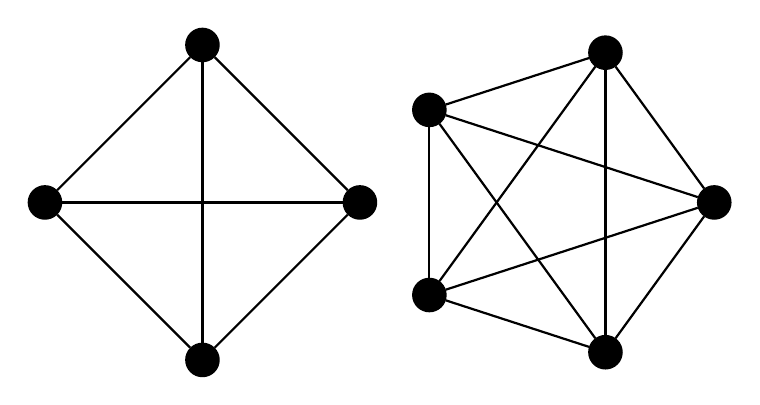
\begin{tikzpicture}[scale=0.5]

\GraphInit[vstyle=Simple]

\begin{scope}[xshift=0 cm]
\grComplete[prefix=p]{4}
\end{scope}
\begin{scope}[xshift=9 cm]
\grComplete[prefix=q]{5}
\end{scope}

\end{tikzpicture}

  \caption{$K_{4}$ and $K_{5}$}
  \label{fig:complete}
\end{figure}

A \emph{one-factor} $f_i$ is a set of edges in which each vertex appears exactly once.

\begin{example}
Two possible one-factors of $K_4$ are:
$$f_1 = \{12,34\},\, f_2 = \{13,24\}$$
\end{example}

\begin{figure}
  \centering
  \input{figure/two-one-factors}
  \caption{Two one-factors of $K_{4}$}
  \label{fig:two-one-factors}
\end{figure}

A \emph{one-factorisation} of the complete graph is a set of one-factors in which all possible edges (i.e. all unordered pairs from the edge-set) appear exactly once.

\begin{figure}
  \centering
  \input{figure/k6-factorisation}
  \caption{$K_{6}$ and a one-factorisation of $K_{6}$}
  \label{fig:k6-factorisation}
\end{figure}

\begin{example}
Here
$G = K_6$
the complete graph on six vertices with
$$V = \{1, 2, 3, 4, 5, 6\}$$
$$E = \{12, 13, 14, 15, 16, 23, 24, 25, 26, 34, 35, 36, 45, 46, 56\}$$
The one-factors are

$$
f_1 = \{12, 35, 46\} \hspace{0.5cm}
f_2 = \{14, 23, 56\} \hspace{0.5cm}
f_3 = \{16, 25, 34\} \hspace{0.5cm}
f_4 = \{13, 26, 45\} \hspace{0.5cm} 
f_5 = \{15, 24, 36\}
$$
because
$f_1 \cup f_2 \cup f_3 \cup f_4 \cup f_5 = E$,
$F = \{f_1, f_2, f_3, f_4, f_5\}$
is a one-factorisation of
$G$,
shown in Figure~\ref{fig:k6-factorisation}.
\end{example}

Two one factors $f$ and $l$ are said to be \emph{orthogonal} if $f \cap l$ contains at most one edge.
Two one-factorisations $F$ and $L$ are orthogonal if every one-factor in $F$ is orthogonal to every one-factor in $L$.

Once again consider the square array in \eqref{eq:roomsquare}.
If the individual elements within the array constituted the vertex set of a graph (call it $R$) and the pairs within each box of the array were edges, we know that each row is a one-factor and each column is a one-factor (because each member of $R$ occurs precisely once in each row and once in each column).

Furthermore, because all edges from the edge-set of the complete graph (i.e. all unordered pairs from $R$) appear once within the array, we know that the rows together form a one-factorisation and the columns form another, different, one-factorisation of $K_8$.
Also, because any row factor intersects any column factor in only one pair (edge), all the row factors are orthogonal to all the column factors and hence the two one-factorisations are orthogonal.
We have demonstrated the following theorem, given in
\cite{dinitzContemporaryDesignTheory1992}
and proven in
\cite{nemethStudyRoomSquares1969}.

\begin{theorem}
The existence of a Room square of side $n$ is equivalent to the existence of two orthogonal one-factorisations of the complete graph $K_{n+1}$.
\end{theorem}

An example is given in Figure \ref{fig:kirkmans-square} based on the Room square in \eqref{eq:roomsquare}

\begin{figure}
  \centering
  \input{figure/kirkmans-square}
  \caption{Two orthogonal one-factorisations of $K_{8}$ based on Kirkman's square of 1850.}
  \label{fig:kirkmans-square}
\end{figure}

\section{Hill-Climbing Algorithm for Room Squares}
  The idea behind hill-climbing algorithms is to suppose there exists a \emph{neighbourhood} of feasible solutions to some problem \emph{instance}.
With each \emph{feasible} solution there is an associated \emph{cost} (or profit) and finding an optimal solution becomes a matter of finding the solution with minimum cost (or maximum profit).

A hill-climbing algorithm non-deterministically selects a solution from the neighbourhood system such that the cost is less than that of some initial solution until its procedure fails, hence finding the locally optimal solution.



\input{main/03_existence_proof}
\chapter{An Existence Theorem for Room Squares}
\label{ch:existence-theorem}

\begin{theorem}
There exists a Room square of side $v$, where $v$ is a positive integer different from 3 or 5.
\end{theorem}

\begin{proof}
A Room square of side one exists trivially.

Any positive integer can be rewritten in the form:

\begin{equation}
v = 3^{a}5^{b}n
\end{equation}

where $n$ is relatively prime to fifteen, i.e.  $(15, n) = 1$.

Suppose that $a + b = 0$, then a Room square exists due to Theorems
\ref{thm:starter-adder},
\ref{thm:furnishing},
\ref{thm:strong-starter-3},
\ref{thm:chong-chan},
\ref{thm:multiply},
and
\ref{thm:wallis}.

For $a + b = 1$, then either $v = 3n$ or $v = 5n$.

In both cases, provided $v > 5$, Theorem \ref{thm:wallis} guarantees the existence of a Room square of side $v$.

Now consider $a + b = 2$.
There are three cases.

\begin{enumerate}
  \item{$v = 3\cdot 5\cdot n$}
  \item{$v = 3^{2}n$}
  \item{$v = 5^{2}n$}
\end{enumerate}

In all cases, a Room square exists by Theorem \ref{thm:wallis}, provided that Room squares of side nine, fifteen and twenty-five all exist.

A Room square of side twenty-five exists by Theorem \ref{thm:strong-starter-3} and Room squares of side nine and fifteen were constructed in
\cite{mullinFurnishingRoomSquares1969}

For examples of Room squares of orders ten and sixteen see, respectively, XXXX and XXX.

Greater values of $a + b$ follow by induction since if $a + b \geq 3$, where $t = 3^{c}5^{d}n$ and $c + d \geq 2$.
In both cases applying Theorem \ref{thm:wallis} will provide a square of side $v$ given one of side $t$.

\end{proof}

\chapter{Balanced Room Squares}
\label{ch:balanced-room-squares}

\section{BIBDs and BRSs}

A \inlinedef{balanced incomplete block design} (BIBD) is an arrangement of elements (varieties) from a set $S$ of size $v$, into $b$ subsets (blocks) each of size $k$ such that each variety occurs in $r$ blocks and any particular pair of distinct varieties occurs in $\lambda$ blocks.

\begin{example}
\begin{equation}
\label{eq:bibd}
\{a,b,c\},\{a,b,d\},\{a,c,e\},\{a,d,f\},\{a,e,f\},\{b,c,f\},\{b,d,e\},\{b,e,f\},\{c,d,e\},\{c,d,f\}
\end{equation}
\eqref{eq:bibd} is a BIBD with parameters $v = 6$, $b = 10$, $k = 3$,
$r = 5$, $\lambda = 2$.
\end{example}

In any $\BIBD(v, b, r, k, \lambda)$ there are $b$ blocks each containing $k$ elements, so $bk$ elements in total.
Also, each of the $v$ elements occurs $r$ times, so there are $rv$ elements in total.
Therefore
\begin{equation}
bk = vr
\end{equation}

Also in a particular block, any element makes a pair with $k - 1$ other elements, and each element occurs in $r$ blocks, so there are $r(k - 1)$ pairs involving that element.
Also, by definition, that element is paired with each of the other $v - 1$ members of $S$ $\lambda$ times, so:
\begin{equation}
\lambda (v - 1) = r(k - 1)
\end{equation}

The second expression rearranges to give $r = \lambda (v - 1)/(k - 1)$, which can be substituted into the first expression to give $b = v\lambda (v - 1)/k(k - 1)$.
So $b$ amd $r$ are both determined by the values of $v$, $k$ and $\lambda$.
For this reason we need only quote those three parameters when referring to a particular block design.
The example was a $\BIBD(6, 3, 2)$ (or $(6, 3, 2)$-design).

In any Room square, the pairs $\{x, y\}$ are unordered.
If we replace these pairs by one of the ordered pairs $(x, y)$ or $(y, x)$ we call the resulting array an \inlinedef{ordered Room square} (ORS).

Consider the following ordered Room square:
\begin{equation}
  \begin{bmatrix}
    \infty 0 &    62    &    54    &            &    31    &            &          \\
             & \infty 1 &    03    &     65     &          &     42     &          \\
             &          & \infty 2 &     14     &    06    &            &    53    \\
      64     &          &          &  \infty 3  &    25    &     10     &          \\
             &    05    &          &            & \infty 4 &     36     &    21    \\
      32     &          &          &            &          &  \infty 5  &    40    \\
      51     &    43    &    20    &     20     &          &            & \infty 6 \\
  \end{bmatrix}
  \label{eq:ors}
\end{equation}

Suppose we extract the blocks of a design (not necessarily a BIBD) from this square in one of the two following ways:

\begin{enumerate}
 \item{As \emph{half-columns}. This means taking all left hand
    members of pairs from a particular column as the members
    of one block, and all right hand members as another
    block.}
 \item{By \emph{half-rows}. Take all left members from a particular
    row as one block, and all right members as another
    block.}
\end{enumerate}

Notice that for this example, both methods generate exactly the same blocks.

\begin{equation}
\begin{split}
\{\infty,6,5,3\},\{0,2,4,1\},\{\infty,0,6,4\},\{1,3,5,2\},\{\infty,1,0,5\},\{2,4,6,3\},\{6, \infty,2,1\}, \\
\{4,3,5,0\},\{0,\infty,3,2\},\{5,4,6,1\},\{3,1,\infty,4\},\{2,6,5,0\},\{5,4,2,\infty\},\{1, 3,0,6\}
\end{split}
\end{equation}

Certainly this design seems to have the appropriate parameters to qualify as a BIBD.
The original Room square was based on eight elements, hence $v = 8$.
Also, the Room square’s seven rows each produced two blocks of four elements, hence $b = 14$ and $k = 4$.

Finally, each element occurred once in each row of the Room square, therefore in half the total number of blocks, hence $r = 7$.

\begin{equation}
bk = 4\cdot 14 = 7 \cdot 8 = vr
\end{equation}

So this design is a BIBD, provided:
\begin{equation}
\lambda = \frac{r(k - 1)}{v - 1} = \frac{7(3)}{7} = 3
\end{equation}

In other words, provided each pair of elements occurs in precisely three blocks.

By definition a \inlinedef{balanced Room square} $\BRS(n)$ is an ordered Room square based on $n$ elements whose corresponding block design, derived as above, is a BIBD.

\section{Complete Balanced Howell Rotations}

Edwin C. Howell is an enigmatic figure in the history of mathematics.
The rotations named after him are designs for the scheduling of bridge tournaments.

In a duplicate bridge tournament players compete in partnerships, two partnerships at a table.
At the beginning of a round each table is given one from a certain number of duplicate boards each of which contains a pack of cards dealt evenly into four pockets.
The boards are labelled north-south-east-west, and are aligned on the table so that one partnership plays north-south and the other east-west.
After the game is finished the cards are returned to the pockets as they were dealt and the duplicate board is returned, to be used again in subsequent matches.

If one partnership plays directly against another at the same table, the two partnerships are said to \inlinedef{oppose} each other.
If two partnerships play in the same direction on the same board in different rounds, they are said to \inlinedef{compete}.

In scoring, not only is the performance of teams in opposition considered, but also the performance of partnerships which compete.

A good tournament design would have the properties that each partnership opposed each other partnership at the same table exactly once and also that each partnership competed against each other partnership at the same number of times.

A \inlinedef{complete balanced Howell rotation} $\CBHR(n)$\footnote{This definition is extracted in its entirety from [8]} is an array (based on $n$ elements) of side $s$, where $s = n$ for $n$ odd, and $s = n-1$ for $n$ even, which satisfies the following properties:\footnote{Where the blocks are derived in the same way as for a BRS.}
\begin{enumerate}
  \item{Each of the $s^2$ cells is empty or contains an ordered
    pair of distinct elements.}
  \item{Each of the $n$ elements appears exactly once in each
    row and each column. (If $n$ is odd, then one row and
    one column is excepted)}
  \item{Each unordered pair of distinct elements occurs in
    exactly one cell of the array.}
  \item{Each pair of distinct elements appears together in a
    block exactly $\left \lfloor{n/2}\right \rfloor -1$
    times, where $\left \lfloor{x}\right \rfloor$ means the
    integral part of $x$.}
\end{enumerate}

To interpret a CBHR as a duplicate bridge tournament schedule, we represent the partnerships by elements, the boards ny rows and the rounds of the tournament by columns.

Then an ordered pair $(x, y)$ in position $(i, j)$ of the array corresponds to partnership $x$ opposing partnership $y$ on board $i$ in round $j$.
We adopt the convention that $x$ plays NS, $y$ EW.
The third property in the definition of a CBHR ensures that all partnerships are in opposition exactly once, while the fourth (with blocks of the associated BIBD representing partnerships in competition) ensures that each partnership competes against each other partnership the same number of times.

Notice that when $n$ is even the definition of a CBHR is precisely that of a balanced Room square.
So the BRS above is also a $\CBHR(8)$.
The reason for maintaining both definitions is that a CBHR is, according to conditions 2 and 4, allowed to have odd order.
Also, an important construction for $\BRS(4n)$, which will be introduced, involves two $\CBHR(2n - 1)$s.

Unlike Room squares the question of the existence of balanced Room squares is far from resolved, but various proofs have shown there to be many infinite classes of these designs.
The details of some of these proofs are given below.

Interestingly the existence problem for balanced Room squares (then known exclusively as CBHR) was brought to the attention of mathematicians, in
\cite{parkerBalancedHowellRotations1955},
the very same year as T.G. Room published his original article.
Either this problem has proved to be very much more difficult, or has aroused significantly less interest.
The first general result, that of
\cite{hwangMoreContributionsConstructing1970},
coming only a few years before the corresponding problem for Room squares was settled
\cite{wallisExistenceRoomSquares1973}.

In order to discuss these results the first step is to make the necessary adaptation of the starter-adder approach.

\section{Starters and Adders for BRS and CBHR}

In deriving the definitions of a starter and adder for a Room square, the terminology of difference systems was introduced.
We saw that a requirement of the starter was that each non-zero member of the relevant Galois field occurred exactly once as a difference between the members of some pair.
This was so that each pair occurred exactly once in the Room square.

BIBDs can be constructed from difference systems in much the same way, but with the difference that each element in the BIBD occurs occurs with each other element $\lambda$ times, not necessarily just once.

\begin{example}
A BIBD on $GF(7)$ can be constructed from the sets $\{6, 5, 3\}, \{2, 4, 1\}$.

\begin{equation}
\label{eq:left}
\{0, 6, 4\}, \{1, 0, 5\}, \{2, 1, 6\}, \{3, 2, 0\}, \{4, 3, 1\}, \{5, 4, 2\}
\end{equation}
are the blocks obtained from the left hand set.

\begin{equation}
\label{eq:right}
\{3, 5, 2\}, \{4, 6, 3\}, \{5, 0, 4\}, \{6, 1, 5\}, \{0, 2, 6\}, \{1, 3, 0\}
\end{equation}
are the blocks obtained from the right hand set.

Because the two sets are both triples, under cyclic construction the block design obtained will necessarily have $k = r = 3$.

The left hand set \eqref{eq:left} has each non-zero member of $GF(7)$ occurring exactly once as a difference between its members.
So, taken with its translates (those blocks obtained from it under cyclic development), this set should form a BIBD with $r = 3$ and $\lambda = 1$.

Similarly the right hand block \eqref{eq:right} forms a BIBD with $r = 3$ and $\lambda = 1$, and the two sets taken together as difference system therefore generate a BIBD with $r = 6$ and $\lambda = 2$.

If we add the ideal element $\infty$ to the left hand set and all its translates, and 0 to the right hand set (developing it cyclically along with the other members) then we obtain a new BIBD with $r = 7$ and $\lambda = 3$, whose blocks are:
\begin{equation*}
  \begin{split}
  \{\infty,6,5,3\},\{\infty,0,6,4\},\{\infty,1,0,5\},\{\infty,2,1,6\},\{\infty,3,2,0\},\{\infty,4,3,1\},\{\infty,5,4,2\} \\
  \{0,2,4,1\},\{1,3,5,2\},\{2,4,6,3\},\{3,5,0,4\},\{4,6,1,5\},\{5,0,2,6\},\{6,1,3,0\}
  \end{split}
\end{equation*}

Which is precisely the BIBD obtained from the Room square at the beginning of this chapter.
\end{example}

If the block design associated with a BRS, or a CBHR, is obtained by taking the left hand member of the pairs in the first row as one block and the left hand members in subsequent rows as the translates, and all right members of pairs as the remaining blocks of a BIBD, then clearly those two blocks, the left hand and the right hand, which belong to the starter must form a difference system.

The set of pairs $(x_1, y_1), (x_2, y_2), \ldots, (x_{n - 1}, y_{n - 1})$ is a \inlinedef{balanced starter} in $G = GF(2n - 1)$ if:
\begin{enumerate}
  \item{the unordered pairs $\{x_i, y_i\}$ form a starter in
    $G$, and} \label{cond1}
  \item{the blocks $\{x_1, x_2, \ldots, x_{n - 1}\}$ and
    $\{y_1, y_2, \ldots, y_{n - 1}\}$ form a difference system.} \label{cond2}
\end{enumerate}

A balanced starter is \inlinedef{strong} if $x_1 + y_1, x_2 + y_2, \ldots, x_{n - 1} + y_{n - 1}$ are all distinct modulo $(2n - 1)$.

\begin{theorem}
Given a strong balanced starter on $G = GF(2n - 1)$, then a $\CBHR(2n - 1)$ exists.
\end{theorem}

\begin{proof}
Assign the pair $(x_i + g, y_i + g)$ to cell $(g, x_i + y_i + g)$ for all $g \in G$.

Condition \ref{cond1} along with the strong-ness of the starter ensures that every $g \in G$ occurs in every row and column exactly once except $g$ does not occur in row or column $g$ for all $g \in G$ [due to the absence in cell
$(0, 0)$ of the pair $\{\infty, 0\}$].

Condition \ref{cond1} also ensures that each unordered pair of $G$ occurs exactly once in the array, replace the unordered pairs with ordered pairs.

That the block design obtained is balanced follows from condition \ref{cond2}.

Notice that each of the two blocks generates $(n - 1)(n - 2)$ differences and these represent each of $2n - 2$ members of $G \backslash \{0\}$, $\lambda$ times.
Therefore $2(n - 1)(n - 2) = \lambda (2n - 2)$ which implies $\lambda = n - 2$.
\end{proof}

\begin{theorem}
Given a strong balanced starter on $G = GF(2n - 1)$, then a $\BRS(2n)$ exists.
\end{theorem}

\begin{proof}
Assign the pair $(x_i + g, y_i + g)$ to cell $(g, x_i + y_i + g)$ for all $g \in G$, and (provided $n$ is even), also assign the pair $(\infty, g)$ to cell $(g, g)$ for all $g \in G$.

Again, condition \ref{cond1} and the strong-ness of the starte r ensure that an ORS based on $G \cup \{\infty\}$ is obtained.
The block design associated with this array has initial blocks, $\{\infty\} \cup \{x_1, x_2, \ldots, x_{n - 1}\}$ and $\{0\} \cup \{y_1, y_2, \ldots, y_{n - 1}\}$.

Adjoining 0 to $\{y_1, y_2, \ldots, y_{n - 1}\}$ creates each non-zero member of $G$ as a difference once more, either as $y_i - 0$ or $0 - y_i$.

Adjoining $\infty$ to $\{x_1, x_2, \ldots, x_{n - 1}\}$ creates $n - 1$ pairs involving $\infty$ in this block, hence $\infty$ makes a pair with each member of $G$ $n - 1$ times.
So the design is balanced with a concurrence number of $n - 1$.

It is a simple matter to derive the remaining parameters of the BIBD associated with either array.

\begin{tabular}{cccccc}
                   &    $v$   &     $b$     &    $r$     &   $k$   & $\lambda$  \\ \hline
      $\CBHR(2n-1)$ & $2n - 1$ & $2(2n - 1)$ & $2(n - 1)$ & $n - 1$ &  $n - 2$   \\
$\CBHR(2n)/\BRS(2n)$ &   $2n$   & $2(2n - 1)$ &  $2n - 1$  &   $n$   &  $n - 1$
\end{tabular}

The block design of a balanced Room square is \emph{self-complementary}.
This means that if a block $D$ belongs to the design, then its complement $\overline{D}$ also appears.
If the left hand pairs in row $x$ form one block then the right hand pairs in the same row are also a block, and the two blocks are complementary.
Alternatively we can say that, in a self-complementary BIBD, the complementary design (obtained by replacing all blocks with their complements) is identical to the design itself.
\end{proof}

\cite{schellenbergBalancedRoomSquares1972}
proved an interesting result regarding self-complementary BIBDs.

\begin{theorem}
In a self-complementary BIBD with parameters of the form, $(2n, 2(2n - 1)t, (2n - 1)t, n, (n - 1)t)$, every triple of elements is contained in $t(n - 2)/2$ blocks.
\end{theorem}

\begin{proof}
Suppose $B$ is a self-complementary BIBD with parameters of the form above, based on a set of elements $V$.
Denote by $S_{i\ldots j}$ the set of blocks which contain $u$ but not $v$ or $w$.
Because the design is self-complementary to each block of this set there corresponds a unique block which contains $v$ and $w$ but not $u$.
The set of these blocks is $S_{vw} - S_u$ and clearly
\begin{equation}
|S_u - \{S_v \cup S_w\}| = |S_{vw} - S_u|
\end{equation}

Now,
\begin{equation}
|S_u-\{S_v \cup S_w\}| = |S_u| - |S_{uv}| -|S_{uw}| + |S_{uvw}|
\end{equation}
and,
\begin{equation}
|S_{vw} - S_u| = |S_{vw}| - |S_{uvw}|
\end{equation}

Therefore
\begin{equation}
|S_u| - |S_{uv}| -|S_{uw}| + |S_{uvw}| = |S_{vw}| - |S_{uvw}|
\end{equation}
and so
\begin{equation}
2|S_{uvw}| = |S_{vw}| + |S_{uv}| + |S_{uw}| - |S_{U}|
\end{equation}

Because $B$ is a $\BIBD$, each pair of elements occur together in $\lambda = (n - 1)t$ blocks and each element occurs in $r = (2n - 1)t$ blocks.
So,
\begin{equation}
|S_{vw}| = |S_{uv}| = |S_{uw}| = (n - 1)t
\end{equation}
and
\begin{equation}
|S_u| = (2n - 1)t
\end{equation}

Therefore,
\begin{equation}
2|S_{uvw}| = 3(n - 1)t - (2n  -1)t = (n - 2)t
\end{equation}
and so,
\begin{equation}
|S_{uvw}| = \frac{(n - 2)t}{2}
\end{equation}

Since $u$, $v$ and $w$ are arbitrary this implies that each triple occurs in $(n - 2)t/2$ blocks.
\end{proof}

The implication of this result for balanced Room squares is that, because $t = 1$ for a $\BRS$ \footnote{The $t=1$ case was proven by Stanton and Sprott (1964) and Parker (1963) prior to Schellenberg.} and we require the LHS of this expression to be an integer, $n$ is necessarily even.
So writing $n = 2m$, we know the order of a $\BRS$ is always of the form $4m$.

\begin{corollary}
A $\BRS(n)$ can only exist for $n \equiv 0$ mod 4.
\end{corollary}

We now present Hwang’s starter-adder construction for balanced Room squares.

\begin{theorem}
\label{thm:hwang}
There exists a $\BRS$ of order $q+1$, where $q = p^r \equiv 3\pmod 4$ is a prime power strictly greater than 3.
\end{theorem}

\begin{proof}
We show that the pairs
\begin{equation}
X = \left\{(x^{2i + 1}, x^{2i}): 0 \leq i \leq \frac{q - 3}{2} \right\}
\end{equation}
form a balanced starter, where $x$ is a primitive element in $GF(q)$, and the set
\begin{equation}
A(X) = \left\{-x^{2i}(1 + x): 0 \leq i \leq \frac{q - 3}{2} \right\}
\end{equation}
is a corresponding adder.

We have already shown that the unordered pairs
\begin{equation}
\left\{\{x^{2i}, x^{2i + 1}\}: 0 \leq i \leq \frac{q - 3}{2} \right\}
\end{equation}
are those of a starter with adder $A(X)$.
So it remains to show that the starter is balanced which involves proving that the two blocks
\begin{equation}
B_1 = \{0, x, x^3, \ldots, x^{q - 2}\} \mathrm{and} B_2 = \{\infty, x^0, x^2, \ldots, x^{q - 3}\}
\end{equation}
generate a $\BIBD$.
This result is due to R. C. Bose and makes use of the properties of the squares and non-squares of $GF(q)$ where $q$ is an odd prime.

Let $R$ and $N$ denote the sets of non-zero square and non-squares in $GF(q)$, respectively.

\begin{equation}
R = \{x^2, x^4, \ldots, x^{q - 1}\}
\end{equation}

\begin{equation}
N = \{x^1, x^3, \ldots, x^{q - 2}\}
\end{equation}

These sets both contain precisely $\frac{1}{2}(q - 1)$ elements.

So, $B_1 = \{0\} \cup N$ and because $x^{q - 1} = 1 = x^0$, $B_2 = \{\infty\} \cup R$.
Also, if $a$ is square then $-a$ is a non-square, which implies that $R = -N$.

To show that the blocks with their translates form a $\BIBD$ it is necessary to show that the differences between members of $B_1$ and $R$ generate all the non-zero members of $GF(q)$ some number of times, then by adjoining the element $\infty$ to $R$ and its translates will generate a $\BIBD$.

Firstly, suppose that 1, which belongs to $R$, can be expressed as a difference between members of $R$ in a certain number of different ways,
\begin{equation}
1 = x^{2a_1} - x^{2b_1} = \ldots = x^{2a_r} - x^{2b_r}
\end{equation}

Were this true, any member of $R$ could be written as a difference in the same number of ways.

Multiply through by any $x^{2s} \in R$
\begin{equation}
x^{2s} = x^{2(a_1 + s)} - x^{2(b_1 + s)} = \ldots = x^{2(a_r + s)} - x^{2(b_r + s)}
\end{equation}

But now suppose that any element of $R$ can be expressed as a difference between members of $R$ in a certain number of ways, i.e. assume this second expression holds.
Then by dividing through by $x^{2s}$, we recover the first expression and hence for each representation of 1 there is a corresponding representation of $x^{2s}$, and vice versa.
So there are an equal number of representations of every member of $R$ as a difference of members of $R$.
The remaining non-zero members of $GF(q)$, are all those $q \notin R$ where $-q \in R$, but each representation of $-r$ gives a corresponding representation of $r$:
\begin{equation}
-r = x^{2a} - x^{2b}
\end{equation}
\begin{equation}
r = x^{2b} - x^{2a}
\end{equation}

So every element of $-r$ has the same number of representations as a difference between members of $R$ as $R$ does.

We know that $R$ has $\frac{1}{2}(q-1)$ elements, therefore there are
\begin{equation}
\frac{1}{2}(q-1) \cdot \frac{1}{2} (q-3) = \frac{1}{4}(q-1)(q-3)
\end{equation}
differences between those elements,
and if each of these differences generates each of the $q-1$ non-zero members of $GF(q)$ $\lambda$ times then:
\begin{equation}
\lambda(q - 1) = \frac{1}{4}(q - 1)(q - 3)
\end{equation}
and
\begin{equation}
\lambda = \frac{1}{4}(q - 3)
\end{equation}

Also, because $N = -R$, we can say that all the non-zero members of $GF(q)$ arise as differences between members of $N$.
Further, $B_1$ also gives the differences $0 - n, n - 0$ for all $n\in N$, which are all the non-zero members of $GF(q)$, once again.
So in total every non-zero member of $GF(q)$ occurs as a difference between elements of $B_1$ and $R$, $2 \cdot \frac{1}{4}(q - 3) + 1 = \frac{1}{2} (q - 1)$ times.
Because $R$ and its translates each contain $\frac{1}{2}(q - 1)$ elements, each member of $GF(q)$ occurs $\frac{1}{2}(q - 1)$ times in all those blocks.
Therefore, adjoining $\infty$ to each block generates blocks of size $\frac{1}{2}(q - 1)$, with $\infty$ making a pair with each member of $GF(q)$, $\frac{1}{2}(q - 1)$ times.
So we can say that $B_1$, $B_2$ and their translates for a $\BIBD(q  +1, \frac{1}{2}(q + 1), \frac{1}{2}(q - 1))$.
Therefore Hwang’s starter is balanced. 
\end{proof}

The $\BRS$ in \eqref{eq:ors} was obtained from Hwang’s starter, hence its block design is a $\BIBD$.

\begin{example}
A balanced starter in $GF(19)$ is
\begin{equation}
X = \{(2,1),(8,4),(13,16),(14,7),(18,9),(15,17),(3,11),(12,6),(10,5)\}
\end{equation}

Which has a corresponding adder:
\begin{equation}
A(X) = \{16,7,9,17,11,6,5,1,4\}
\end{equation}

So the following row is an appropriate choice for a $\BRS(20)$:
\begin{equation}
 \begin{bmatrix}
   0 & - & 14,7 & 2,1 & 15,7 & - & - & - & 18,9 & - & 13,16 & - & 8,4 & - & 3,11 & 10,5 & - & - & 12,6
 \end{bmatrix}
\end{equation}

\end{example}

\section{A Multiplicative Construction for BRS}

Although the Hwang starter-adder construction establishes the existence of an infinite class of $\BRS$, like the Mullin-Nemeth construction for Room squares, exceptions still remain.

Particularly all those $\BRS$ of order $q + 1$ where $q$ is not a prime power, yet is congruent 3 modulo 4.
For example, the existence of $\BRS(16)$ is not established yet, because 15 is not a prime power.

One approach to resolving this problem would be to establish a multiplication theorem like those established for Room squares.
The following doubling construction for $\BRS$ (due to Schellenberg), for example, enables to construction of a $\BRS(16)$ from two $\BRS(8)$.

Significantly, used along with Hwang’s starter-adder construction, it establishes the existence of another infinite class of $\BRS$, those of order $2(q + 1)$, where $q$ is subject to the conditions of Theorem \ref{thm:hwang}.

Before presenting the doubling construction a few definitions need to be made, and another result regarding self-complementary block designs established.

The \inlinedef{reduced} Room square $\hat{R}$, is obtained by taking a standardised Room square $R$ and removing the pairs involving $\infty$, i.e. the diagonal pairs.

Two $ORS$, $R$ and $S$ (both of side $a$) are said to be a \inlinedef{Latin pair} if on forming the join of $\hat{R}$ and $\hat{S}$, and placing the pair $(i, i)$ in cell $(i, i)$ for $0 \leq i \leq q - 1$ the join of two $MOLS$ is obtained, denoted by $R \odot S$.

A \inlinedef{common traversal} of $R \odot S$ is a set of $q$ cells, one from each row and each column, whose $n$ ordered pairs have $n$ distinct first elements and $n$ distinct second elements.

Suppose we have a set of varieties $V = \{1, 2, 3, \ldots\}$, then by a set $V'$, we mean $V'=\{1', 2', 3', \ldots\}$.

\begin{lemma}
If
\begin{equation}
  \bigcup\limits_{i=1}^{2k-1} \left \{C_i,\bar{C_i} \right \} 
  \qquad \bigcup\limits_{i=1}^{2k-1} \left \{D_i,\bar{D_i} \right \}
\end{equation}
are the blocks of two self-complementary $\BIBD$s, both defined on a set of elements $V$, where $\bar{C}$ denotes the complement of $C$, with parameters $(2k, 2(2k - 1), 2k - 1, k, k-1)$ then.

\begin{equation}
\bigcup\limits_{i=1}^{2k-1} \left \{C_i \cup D'_i, \bar{C_i} \cup \bar{D'_i}, C_i \cup \bar{D'_i}, \bar{C_i} \cup D'_i  \right \} \cup \{V,V'\}
\end{equation}
is the set of blocks of a self-complementary $\BIBD$, defined on the set of elements $V \cup V'$, with parameters $(4k, 2(4k - 1), 4k - 1, 2k, 2k - 1)$.
\end{lemma}

\begin{proof}
Consider an arbitrary pair $\{a, b\}$ in the new $\BIBD$ where $a, b \in V$.
The concurrence number of the original $\BIBD$ was $k - 1$, so this pair occurred $k - 1$ times in the blocks
\begin{equation}
\bigcup\limits_{i = 1}^{2k - 1} \left\{C_i, \bar{C_i} \right\}
\end{equation}
but these blocks clearly appear twice each in the new $\BIBD$.
Also the pair $\{a, b\}$ occurs once in the block $V$, so the pair $\{a, b\}$ occurs $2(k - 1) + 1 = 2k - 1$ times.
The same would be true for any pair $\{a, b\}$ when $a, b \in V'$.

Now consider an arbitrary pair $\{a, b\}$ when $a \in V$, and $b \in V'$.
From the definition of complementary blocks $a$ occurs either $C$ or $\bar{C}$ and $b$ in either $D'$ or $\bar{D'}$, for some value of $i$, and because all pair combinations between $C$-blocks and $D'$-blocks are formed in the new design and because $i$ takes $2k - 1$ values in the new design so the pair makes $2k - 1$ appearances.

Hence the new block design is a $\BIBD$ with $\lambda = 2k - 1$.
\end{proof}

\begin{theorem}
\label{thm:schellenberg}
Suppose we have two $\BRS(q+1)$, $R$ and $S$ based on $G = GF(q)$, with the following properties:
\begin{enumerate}
  \item{$R$ and $S$ are a \emph{latin pair} such that}
  \item{$R \odot S$ has a pair of disjoint \emph{common transversals}
    $T_1$ and $T_2$ (with $T_2$ in $R$), which do not
    intersect the main diagonal, and}
  \item{the block designs obtained from $R$ and $S$, call them
    $D(R)$ and $D(S)$ respectively, have the property that
    if $\{\infty\} \cup B_i$ and $\{i\} \cup C_i$ are the
    blocks of $D(R)$ obtained from row $i$, then $\{i\} \cup
    B_i$ and $\{\infty\} \cup C_i$ are the blocks of $D(S)$
    obtained from row $i$.}
\end{enumerate}

Then a $\BRS(2(q + 1))$ exists.
\end{theorem}

\begin{proof}
Define $A$ to be the array obtained from the superposition of $\hat{R}$ and $\hat{S'}$.
Where $\hat{S'}$ is obtained by replacing the elements of $G$ in $\hat{S}$ (the reduced RS) by the corresponding elements of $G'$ and replacing $\infty$ by $\infty'$.
$R$ and $S$ were $\BRS$ so each column and row of $A$ contains each member of $G \cup G' \cup \{\infty, \infty'\}$, except those elements $i,i',\infty$ and $\infty'$ which are missing from row and column $i$ due to the reduction process.
Further, $A$ contains every pair $\{i,j\},\{i',j'\} i,j \in G,i \neq j$ exactly once.
Define $B$ as the array obtained from $R \odot S$ when each pair $(i,j)$ is replaced by $(i, j')$.

Now, $D$ is defined as the array obtained from $B$ according to this procedure.

If cell $(m, n), m\neq n$ of $R$ is not empty, replace $(i, j')$ in cell $(m, n)$ of $B$ by $(j', i)$.
Because $R \odot S$ is a pair of superposed orthogonal latin squares $D$ contains each member of $G \cup G'$ exactly once in each row and column.
Also, the way in which we have repalced elements ensures that every unordered pair $\{i, j'\}$ for all $i, j \in G$ occurs exactly once in $D$.

Next, construct $C$ by arranging the arrays $A$ and $D$ according to the following layout, in which $\phi$ is the $q \times q$ array with every cell empty, $\theta$ the $1 \times q$ array of empty cells and $\theta ^T$ the transpose of $\theta$
\begin{equation}
  C =
  \begin{bmatrix}
    A & \phi & \theta^T \\
    \phi & D & \theta^T \\
    \theta & \theta & (\infty',\infty)
  \end{bmatrix}
\end{equation}

The rows and columns of this new array are labelled $0, 1, 2, \ldots, q - 1, 0', 1', 2', \ldots, (q - 1)',l$.
So that the pair $(\infty ', \infty)$ is in cell $(l, l)$.

Let
\begin{equation}
 T'_p = \{ (i'_m,j'_m) | (i_m,j_m) \text{ is a cell transversal } T_p \}
\end{equation}
be the set of cells of $C$, corresponding to transversal
$T_p (p=1,2)$ of $R \odot S$.

Construct a new array $F$, based on $C$ according to the following prescription:

Consider cell $(i'_m, j'_m) \in T'_1$. If cell $(i_m, j_m)$ is not empty in $R$ then $(i'_m, j'_m)$ of $C$ contains a pair $(k', n)$, otherwise it contains a pair $(n, k')$. [In either case $k, nm \in G k \neq n$ (the transversal does not intersect the diagonal)].
Remove whichever pair appears in cell $(i'_m, j'_m)$ and put it in cell $(i'_m, l)$.
Also place $(\infty', k')$, $(\infty, n)$ in cells $(k, j'_m), (n, j'_m)$ respectively.

If $(i'_m, j'_m) \in T'_2$ then a pair $(k', n)$ appears in cell $(i'_m, j'_m)$.
Again remove it, but this time put it in $(l, j'_m)$.
In addition pairs $(k', \infty), (\infty ', n)$ go in cells $(i'_m, k), (i'_m, n)$ respectively.

$F$ is a $\BRS$ because,
\begin{itemize}
  \item{$A$ and $D$ between them intially contain all the
    unordered pairs $\{i, j\}, \{i', j'\}$
    $i, j \in G, i\neq j$ and
    $\{i,j'\}$ for all $i,j \in G$. So $F$ has an
    ordered pair corresponding to each of these.}
  \item{The procedure in the preceding paragraph contributes
    the remaining ordered pairs
    $(\infty', k'),(\infty,n),(k',\infty),(\infty ',n)$ for all $k,n \in G k \neq n$
    in such a way that the
    elements missing from the first $q$ rows and columns are
    suitably placed, and $\infty$ and $\infty '$ are placed
    in each row and column of $F$.  Hence each row and
    column of $F$ contains every member of
    $\{\infty, \infty '\} \cup G \cup G'$
    exactly once.}
\end{itemize}

The block design obtained from the rows of $F$ has blocks
\begin{equation}
\left.
\begin{split}
\{\infty\} \cup B_i \cup \{\infty'\} \cup C'_i \\
\{i\} \cup C_i \cup \{i'\} \cup B'_i
\end{split}
\right \}
0 \leq i \leq q-1
\end{equation}
from rows $0, 1, \ldots, q - 1$ blocks
\begin{equation}
\left.
\begin{split}
\{\infty\} \cup B_i \cup \{i'\} \cup B'_i \\
\{i\} \cup C_i \cup \{\infty\} \cup C'_i
\end{split}
\right \}
0 \leq i \leq q-1
\end{equation}
from rows $0', 1', \ldots, (q - 1)'$, and the blocks
\begin{equation}
\{\infty\} \cup G, \{\infty '\} \cup G'
\end{equation}
obtained from row $l$.

According to condition 3 of Theorem \ref{thm:schellenberg}, these blocks for a $\BIBD$.
\end{proof}

Schellenberg applied his multiplicative construction to the $\BRS$ generated by Hwang’s starter-adder construction, and in doing so was able to establish the following.

\begin{theorem}
For $q \equiv 3\pmod 4$, with $q$ a prime power strictly greater than 3, there exists a $\BRS(2(q+1))$.
\end{theorem}

\begin{proof}
Construct $R$ from the following balanced starter,
\begin{equation}
X = \left \{ (x^{2i},x^{2i+1}):0 \leq i \leq \frac{q-3}{2} \right \}
\end{equation}
with adder,
\begin{equation}
A(X) = \left \{ -x^{2i}(1+x):0 \leq i \leq \frac{q-3}{2} \right \}
\end{equation}

Clearly this is just the Hwang starter-adder of Theorem \ref{thm:hwang}, although the elements in the starter pairs have swapped order.

Now, construct $S$ from the balanced starter,
\begin{equation}
Y = \left \{ (x^{2i-1},x^{2i}):0 \leq i \leq \frac{q-3}{2} \right \}
\end{equation}
\begin{equation}
A(Y) = \left \{ -x^{2i-1}(1+x):0 \leq i \leq \frac{q-3}{2} \right \}
\end{equation}
$Y$ has been obtained simply by swapping the pairs of $X$ and multiplying them by $x^{-1}$.
Therefore, that $Y$ is a balanced starter follows from the fact that $X$ is balanced, as was established in Theorem \ref{thm:hwang}.

It remains to show that $R$ and $S$ satisfy conditions 1, 2 and 3 of Theorem \ref{thm:schellenberg}.
\begin{enumerate}
  \item{$R$ and $S$ are a Latin pair. The positions of the
      starter pairs in the first row of each square are
      determined by the adder, so
      $A(X) \cap A(Y) = \varnothing$ ensures that each
      cell of the first row, hence subsequent rows, of
      $R \odot S$ contains only one pair.
      
      That $R \odot S$ is a pair of superposed Latin squares
      requires that for the pairs in any row, the left hand
      members take all values $0,\ldots, q - 1$, and the right
      members also take values $0,\ldots, q - 1$.  Clearly this
      property holds for all rows if it holds for the first.
      The pairs in the first row of $R \odot S$ are
      \begin{equation}
        \{(0, 0)\} \cup \left \{ (x^{2i - 1}, x^{2i}), (x^{2i}, x^{2i + 1}) \,|\, 0 \leq i \leq \frac{q - 3}{2} \right \}
      \end{equation}
      
      So all $(q - 1)/2$ non-squares and all $(q - 1)/2$
      squares occur as left hand members of pairs, and
      similarly as right hand members. So $R \odot S$ is a
      pair of superposed Latin squares.
      
      For these Latin
      squares to be orthogonal requires that there is no
      repetition of ordered pairs.  For a repetition to
      occur would require some repetition of ordered
      differences among the starter pairs.  Either:
      \begin{equation}
        x^{2i - 1} - x^{2i} = x^{2i} - x^{2i + 1}
      \end{equation}
      or
      \begin{equation}
        x^{2i} - x^{2i-1} = x^{2i+1} - x^{2i}
      \end{equation}
      In other words,
      \begin{equation}
       \pm (x^{2i - 1} + x^{2i + 1}) = \pm (x^{2i} + x^{2i})
      \end{equation}
      Therefore,
      \begin{equation}
        x^{-1} + x = 2
      \end{equation}
      and so $x = 1$.

      Clearly false, so ordered differences are unique.}
  \item{$R \odot S$ has a pair of disjoint \emph{common transversals}.
      For any fixed non-zero $j$ the cells
      $(i, i + j)$, $0 \leq i \leq q - 1$ form a common
      transversal which does not intersect the diagonal.}
  \item{The block designs for $R$ and $S$ are balanced. The
      starters $X$ and $Y$ are balanced starters hence the
      block designs for $R$ and $S$ are $\BIBD$s.}
  \end{enumerate}
\end{proof}

So the Schellenberg multiplication construction establishes the existence of some new orders $q + 1$ where $q$ is not necessarily a prime power. e.g. the orders in bold are now established which had not been under Hwang’s construction:

\begin{center}
  \begin{tabular}{|c|c|c|c|c|c|c|c|c|c|c|c|}
  \hline
     Hwang     &  8 & 12 &    & 20 & 24 & 28 & 32 &    &    & 44 & 48 \\ \hline
  Schellenberg & \textbf{16} & 24 & 32 & \textbf{40} & 48 & \textbf{56} & \textbf{64} & 72 & 80 & \textbf{88} & \textbf{96} \\ \hline
  \end{tabular}
\end{center}

Even with both these theorems, there are obviously missing orders.
The first exception, 36 occurs, for example, because 35 is not a prime power and because 17 is not congruent to 3 modulo 4.

Schellenberg applied the multiplicative construction to the case when $p^r \equiv 1\pmod 4$ [then, of course, $2(p^r + 1) \equiv 0\pmod 4$ as is required] and was able to obtain further results.
Although, as an interesting parallel to the Mullin-Nemeth construction, he also had problems with the Fermat primes and again they were treated separately.
Rather than look at his approach we consider the later approach by Du, Yu, Hwang and Kang amongst others.

\subsection{Symmetric Skew Balanced Starters}

If $(x_1, y_1), (x_2, y_2),\ldots, (x_{(q - 1)/2}, y_{(q - 1)/2})$ are the pairs of a balanced starter in $GF(q)$ then we say that starter is \inlinedef{skew} if $\pm(x_1 + y_1), \pm(x_2 + y_2),\ldots, \pm(x_{(q - 1)/2}, y_{(q - 1)/2})$ are all distinct mod $q$.

Notice that a skew starter is necessarily a strong starter (all sums are distinct).
A balanced starter is \inlinedef{symmetric} if $\{x_1, x_2,\ldots, x_{(q - 1)/2}\} = \{-x_1, -x_2,\ldots, x_{(q - 1)/2}\}$

\cite{hwangCompleteBalancedHowell1984} claimed that Schellenberg’s multiplication theorem could be applied to two $\CBHR(2n - 1)$s, both obtained from $SSBS$, to construct a $\BRS(4n)$.
It was then shown that $SSBS$ exist for all prime powers $2n - 1 = 8k + 5 > 5$, and so the existence of $\BRS(4n)$ for these values was believed to be established.

\begin{center}
\begin{tabular}{|c|c|c|c|c|c|c|c|c|c|c|}
\hline
  k  &  1 &  3 &  4 &   6 &   7 &  12 &  13 &  16 &  18 & 19 \\ \hline
$4n$ & 28 & 60 & 76 & 108 & 124 & 204 & 220 & 268 & 300 & 316 \\ \hline
\end{tabular}
\end{center}

\cite{andersonConstructionBalancedRoom1999} noticed a flaw in this approach and corrected it.

Suppose we wished to apply Schellenberg’s construction to two $\CBHR(2n - 1)$s, call them $P$ and $Q$.
Then it would be necessary to make a slight alteration to Theorem \ref{thm:schellenberg} to accomodate the missing diagonal pairs, i.e. $\{\infty, i\}$ from row $i$.

\begin{theorem}
Suppose we have two $\CBHR(2n - 1)$, $P$ and $Q$ based on $G = GF(2n - 1)$, with the following properties:
\begin{enumerate}
  \item{$P$ and $Q$ are a latin pair such that,}
  \item{$P \odot Q$ has a pair of disjoint
    \emph{common transversals} $T_1$ and $T_2$
    (with $T_2$ in $P$), which do not intersect that main
    diagonal, and}
  \item{the block designs obtained from $P$ and $Q$, call
    them $D(P)$ and $D(Q)$ respectively, have the property
    that if $B_i$ and $C_i$ are the blocks from $D(P)$
    obtained from row $i$, then $B_i$ and $C_i$
    are also the blocks of $D(Q)$ obtained from row $i$.}
\end{enumerate}

Then a $\BRS(4n)$ exists.
\label{thm:schellenberg-alt}
\end{theorem}

\begin{proof}
As for Theorem \ref{thm:schellenberg}.
\end{proof}

It was then claimed that the two $\CBHR(2n - 1)$s obtained from a $SSBS$ and its transpose satisfy the three conditions of Theorem~\ref{thm:schellenberg-alt}.
Hence implying the existence of a $\BRS(4n)$.

However, a counter-example was found.

\begin{lemma}
If $p = 8k + 5$ is a prime, $p > 5$, then the pairs
\begin{equation}
(x^{4i}, -x{4i + 1}), (x^{4i + 2}, x^{4i + 1}) \qquad 0 \leq i \leq 2k
\end{equation}
form a $SSBS$ in $GF(p)$, provided $x^2 - 1$ is a square mod
$p$.
\end{lemma}
\begin{proof}
\begin{enumerate}
\item{The elements in the starter pairs are a complete
    replication of $GF(p) \backslash \{0\}$.
    $x^{\frac{1}{2} (q - 1)} = x^{4k + 2} = -1$, therefore we
    can write the pairs as,
    $$(X^{4i}, x^{4(k + i) + 3}), (x^{4i + 2}, x^{4i + 1}) 0 \leq i \leq 2k$$
    All the members of these pairs are clearly unique and
    there are $4(2k + 1) = 8k + 4$ of them, hence they must all of
    $(GF(p) \backslash \{0\}$.}
\item{The differences are similarly a complete replication of
    $GF(p) \backslash \{0\}$. The differences are
    $\pm x^{4i}(x + 1), \pm x^{4i + 1}(x - 1)$, which can be written
    as
    $$x^{4i}(x + 1), x^{4(i + k) + 2}(x + 1), x^{4i + 1}(x - 1), x^{4(i + k) + 3}(x-1)$$
    Which are all unique provided $(x + 1)$ and $(x - 1)$ have
    the same quadratic character (meaning either both of
    neither are squares).  This is true because
    $(x + 1)(1 - x) = x^2 - 1$ is a square.}
\item{The starter is \emph{skew}, (the positive and negative sums
    are all distinct).  The sums are
    $\pm x^{4i}(1 - x), \pm x^{4i + 1}(x + 1)$
    which again are all unique, provided
    $(1 - x)$ and $(x + 1)$ have the same quadratic
    character.  True, because
    $(1 - x)(x  +1) = -(x^2 - 1) = x^{4k + 2}(x^2  -1)$, is a square.}
\item{The starter is \emph{symmetric}.
    Indeed, $-x^{4i} = x^{4(i + k) + 2}$, generates the
    same elements as $x^{4i + 2}$ shifted by $k$ places.}
\item{The associated block design is balanced.  The blocks in
    the first row are, $\{\infty\} \cup R$, due to the left
    hand members (where $R$ is the set of squares).
    $\{0\} \cup N$, due to the right hand members (where
    $N$ is the set of non-squares).
    We can show that these blocks along with their translates
    form a $\BIBD$.
    
    Using an earlier argument, we can say that
    all elements of $R$ are generated as differences of $R$
    from the same number of times (say $\lambda _1$ times).
    Also, a similar argument allows us to say that all the
    elements of $N$ are generated as differences of $R$ the
    same number of times (say $\lambda _2$). Now, of course
    $N = xR$. So we can say that to each difference of
    members of $R$ which generates a square there is a
    difference of $N$ which generates a non-square.
    Therefore every $r \in R$ occurs as a difference in
    $N, \lambda _1$ times. For the same reason every
    $n \in N$ occurs as a difference between members of
    $N, \lambda _2$ times. Therefore, each element of
    $GF(p) \backslash \{0\}$ occurs $\lambda _1 + \lambda _2$
    times as a difference in $R$ or $N$.
    
    Now, $|R| = |N| = 4k + 2$. So each of the two sets, $R$
    and $N$, gives $(4k + 2)(4k + 1)$ differences. Furthermore
    there are $8k + 4$ elements of $GF(p) \backslash \{0\}$,
    and each occurs as a difference
    $\lambda _1 + \lambda _2$ times. So,
    \begin{equation}
    2(4k + 2)(4k + 1) = (\lambda _1 + \lambda _2)(8k + 4)
    \end{equation}
    Therefore, $\lambda _1 + \lambda _2 = 4k + 1$.
    Adjoining 0 to $N$ creates each member of
    $GF(p) \backslash \{0\}$ once again, as either $0-n$ or
    $n-0$.
    Adjoining $\infty$ to $R$, makes $|R| = 4k + 2$ pairs
    involving $\infty$. Therefore, $\{\infty\} \cup R$ and
    $\{0\} \cup N$ and their translates have between them
    each pair from $\{\infty\{ \cup GF(p)$ occurring $4k + 2$
    times. Hence the block design is balanced.}
\end{enumerate}
\end{proof}

\begin{example}
Let $P$ be the $\CBHR(2n - 1)$ obtained from the $SSBS$ in Lemma 3.2 when $p = 13$
\begin{equation}
  (1, 11), (3, 7), (4, 2), (9, 8), (10, 5), (12, 6)
\end{equation}
\end{example}

By the \inlinedef{transpose} $X^T$ of a starter $X$ we mean those pairs in the first column of the square generated by $X$.

In this case, for example, $(1, 11)$ goes in cell $(0, 12)$ therefore will be a pair in the first column $(1 + i, 11 + i)$ in position $(0 + i, 12 + i)$, such that $12 + i = 0\pmod{13}$. $(2, 12)$ goes in $(1, 0)$ hence belongs to the transpose of this starter

In general a starter-pair $(a, b)$ goes in $(0, a  +b)$, so the corresponding transpose-pair will be $(a - a - b, b - a - b) = (-b, -a)$. So the transpose of the above starter is:
$$(2, 12), (6, 10), (11, 9), (5, 4), (8, 3), (7, 1)$$

If we now apply the Schellenberg construction as suggested in
\cite{hwangCompleteBalancedHowell1984}
we obtain $P \odot Q$:
\begin{equation}
  P \odot Q = \left[\begin{array}{*{13}c}
   0,0  & 2,12  & 10,5  & 6,10  & 9,8  & 12,6 &  4,2  & 11,9  &  7,1  & 5,4  &  3,7  &  8,3  & 1,11 \\
   2,12 &  1,1  &  3,0  & 11,6  & 7,11 & 10,9 &  0,7  &  5,3  & 12,10 & 8,2  &  6,5  &  4,8  &  9,4 \\
   10,5 &  3,0  &  2,2  &  4,1  & 12,7 & 8,12 & 11,10 &  1,8  &  6,4  & 0,11 &  9,3  &  7,6  &  5,9 \\
   6,10 & 11,6  &  4,1  &  3,3  & 5,2  & 0,8  &  9,0  & 12,11 &  2,9  & 7,5  & 1,12  & 10,4  &  8,7 \\
   9,8  & 7,11  & 12,7  &  5,2  & 4,4  & 6,3  &  1,9  & 10,1  & 0,12  & 3,10 &  8,6  &  2,0  & 11,5 \\
   12,6 & 10,9  & 8,12  &  0,8  & 6,3  & 5,5  &  7,4  & 2,10  & 11,2  & 1,0  & 4,11  &  9,7  &  3,1 \\
   4,2  &  0,7  & 11,10 &  9,0  & 1,9  & 7,4  &  6,6  &  8,5  & 3,11  & 12,3 &  2,1  & 5,12  & 10,8 \\
   11,9 &  5,3  &  1,8  & 12,11 & 10,1 & 2,10 &  8,5  &  7,7  &  9,6  & 4,12 &  0,4  &  3,2  &  6,0 \\
   7,1  & 12,10 &  6,4  &  2,9  & 0,12 & 11,2 & 3,11  &  9,6  &  8,8  & 10,7 &  5,0  &  1,5  &  4,3 \\
   5,4  &  8,2  & 0,11  &  7,5  & 3,10 & 1,0  & 12,3  & 4,12  & 10,7  & 9,9  & 11,8  &  6,1  &  2,6 \\
   3,7  &  6,5  &  9,3  & 1,12  & 8,6  & 4,11 &  2,1  &  0,4  &  5,0  & 11,8 & 10,10 & 12,9  &  7,2 \\
   8,3  &  4,8  &  7,6  & 10,4  & 2,0  & 9,7  & 5,12  &  3,2  &  1,5  & 6,1  & 12,9  & 11,11 & 0,10 \\
   1,11 &  9,4  &  5,9  &  8,7  & 11,5 & 3,1  & 10,8  &  6,0  &  4,3  & 2,6  &  7,2  & 0,10  & 12,12 \\
  \end{array}\right]
\end{equation}

Although this is the join of two Latin squares, the repetition of ordered pairs means that they are not orthogonal.
An immediate solution might be to reverse the order of half the repeated pairs, but this approach ruins the join of Latin squares property.
\cite{andersonConstructionBalancedRoom1999} developed a theorem to overcome this property.
We present a slight adaptation of this theorem.
\begin{theorem}
Let $p = 8k + 5$ be a prime, $p > 5$.
Then a $\BRS$ of side $2p + 1$ exists.
\end{theorem}

\begin{proof}
Suppose we take $P \odot Q$, and label elements of the pairs from $P$ with subscript 1 and all those from $Q$ with subscript 2.
Then remove the diagonal pairs $(a, a)$, and call this new array $A$.
$A$ contains all the unordered pairs $\{a_1, b_1\},\{a_2, b_2\}$ exactly once.
The first row of $A$ contains the ordered pairs,
$(x_1^{4i}, -x_1^{4i + 1}), (x_1^{4i + 2}, -x_1^{4i + 1})$
due to $P$, and
$(x_2^{4i + 1}, -x_2^{4i}), (x_2^{4i + 1}, -x_2^{4i  +2})$
due to $Q$.

So all the squares subscript 1 appear as left hand members of pairs as do all the non-squares subscript 2.
Also, all the non-squares appear with subscript 1 in the right hand positions and all the squares with subscript 2.

If we denote the set of squares with subscript 1 by $R_1$, and with subscript 2 by $R_2$.
And similarly denote the sets of non-squares as $N_1$ and $N_2$.
Then in $A$, $R_1 \cup N_2$ occupies the left hand positions while $N_1 \cup R_2$ occupies the right.

Now define $B$ as the array of side $p$ whose first row contains the pairs:
\begin{equation}
(x_2^{4i}, -x_1^{4i + 1}), (x_1^{4i + 2}, x_2^{4i + 1}), (-x_2^{4i}, x_1^{4i + 1}), (-x_1^{4i + 2}, -x_2^{4i + 1})
\end{equation}

So in $B$ the left hand positions are occupied by $R_2 \cup R_1$, while the right are occupied by $N_1 \cup N_2$.
In order that all unordered pairs $\{a_1, b_2\}$ occur once in $B$ requires that in the first row all the members of $GF(p)$ occur once as a difference in one of two ways:

Either as $a_1 - b_2$ which are called $(1, 2)$ \inlinedef{mixed differences} or as $b_2 - a_1$, called $(2, 1)$ mixed differences.

Consider $(2, 1)$ mixed differences in the first row, they are:
\begin{align*}
       x^{4i} + x^{4i + 1} &= x^{4i}(1 + x)      \\
      -x^{4i} - x^{4i + 1} &=-x^{4i}(1 + x)      \\
   x^{4i + 1} - x^{4i + 2} &= x^{4i + 1}(1 - x)  \\
  -x^{4i + 1} + x^{4i + 2} &= -x^{4i + 1}(1 - x)
\end{align*}
i.e. $\pm x^{4i}(1 + x), \pm x^{4i + 1}(1 - x)$

Again, these are all of $GF(p)$ provided that $x^2- 1$ is a square.

Now arrange $A$ and $B$ in the following familiar manner to construct an array of side $2p + 1$:
\begin{equation}
\begin{array}{c|c|c}
\hline
      A     &   \phi   &       \theta ^T   \\ \hline
     \phi   &    B     &       \theta ^T   \\ \hline
    \theta  &  \theta  &  \infty _1, \infty _2  \\ \hline
\end{array}
\end{equation}

Next place the missing pairs in a manner similar to the original construction of Schellenberg.
Take a pair $(a_1, b_2)$ from the first row of $B$ in position $(0_2, h_2)$ and consider the cells in transversal $T_1$ of $B$, where $$T_1 = \left \{((0 + g)_2,(h + g)_2) \middle| g \in Z_p \right \}$$
If cell $(i_2, j_2)$ in $T_1$ contains $(n_1, k_2)$,
\begin{itemize}
  \item{put $(n_1, k_2)$ in cell $(i_2, \infty)$}
  \item{also put $(\infty _1, k_2)$ in $(k_1, j_2)$ and
    $(\infty _2, n_1)$ in $(n_1, j_2)$}
\end{itemize}

Now consider the transversal $T_2$ of $B$, where $(u_1, v_2)$ is a pair in $(0_2, l_2)$ and,
\begin{equation}
T_2 = \left \{((0 + g)_2, (l + g)_2) \middle| g \in Z_p \right \}
\end{equation}
If cell $(i_2, j_2)$ in $T_2$ contains $(h_1, m_2)$,
\begin{itemize}
  \item{put $(h_1, m_2)$ in cell $(\infty, j_2)$}
  \item{also put $(\infty _2, m_2)$ in $(0_2, m_1)$ and
    $(h_1, \infty _1)$ in $(0_2,h_1)$}
\end{itemize}

Finally put $(i_1, i_2)$ in $(i_2, i_2)$ for $0 \leq i \leq p - 1$, and put $(\infty _1, \infty _2)$ in cell $(\infty, \infty)$.
\end{proof}

\begin{example}
Continuing from before,

\begin{equation}
A = \left[\begin{array}{c|*{13}c}
 & 0_1 & 1_1 & 2_1 & 3_1 & 4_1 & 5_1 & 6_1 & 7_1 & 8_1 & 9_1 & 10_1 & 11_1 & 12_1\\ \hline
0_1 &  & 2_2 12_2 & 10_1 5_1 & 6_2 10_2 & 9_1 8_1 & 12_1 6_1 & 4_1 2_1 & 11_2 9_2 & 7_2 1_2 & 5_2 4_2 & 3_1 7_1 & 8_2 3_2 & 1_1 11_1\\
1_1 & 2_1 12_1 & & 3_2 0_2 & 11_1 6_1 & 7_2 11_2 & 10_1 9_1 & 0_1 7_1 & 5_1 3_1 & 12_2 10_2 & 8_2 2_2 & 6_2 5_2 & 4_1 8_1 & 9_2 4_2\\
2_1 & 10_2 5_2 & 3_1 0_1 & & 4_2 1_2 & 12_1 7_1 & 8_2 12_2 & 11_1 10_1 & 1_1 8_1 & 6_1 4_1 & 0_2 11_2 & 9_2 3_2 & 7_2 6_2 & 5_1 9_1\\
3_1 & 6_1 10_1 & 11_2 6_2 & 4_1 1_1 & & 5_2 2_2 & 0_1 8_1 & 9_2 0_2 & 12_1 11_1 & 2_1 9_1 & 7_1 5_1 & 1_1 12_2 & 10_2 4_2 & 8_2 7_2\\
4_1 & 9_2 8_2 & 7_1 11_1 & 12_2 7_2 & 5_1 2_1 & & 6_2 3_2 & 1_1 9_1 & 10_2 1_2 & 0_1 12_1 & 3_1 10_1 & 8_1 6_1 & 2_2 0_2 & 11_2 5_2\\
5_1 & 12_2 6_2 & 10_2 9_2 & 8_1 12_1 & 0_2 8_2 & 6_1 3_1 & & 7_1 4_1 & 2_1 10_1 & 11_2 2_2 & 1_1 0_1 & 4_1 11_1 & 9_1 7_1 & 3_2 1_2\\
6_1 & 4_2 2_2 & 0_2 7_2 & 11_2 10_2 & 9_1 0_1 & 1_2 9_2 & 7_1 4_1 & & 8_2 5_2 & 3_1 11_1 & 12_2 3_2 & 2_1 1_1 & 5_1 12_1 & 10_1 8_1\\
7_1 & 11_1 9_1 & 5_2 3_2 & 1_2 8_2 & 12_2 11_2 & 10_1 1_1 & 2_2 10_2 & 8_1 5_1 & & 9_2 6_2 & 4_1 12_1 & 0_2 4_2 & 3_1 2_1 & 6_1 0_1\\
8_1 & 7_1 1_1 & 12_1 10_1 & 6_2 4_2 & 2_2 9_2 & 0_1 12_1 & 11_2 2_2 & 3_1 11_1 & 9_1 6_1 & & 10_2 7_2 & 5_1 0_1 & 1_2 5_2 & 4_1 3_1\\
9_1 & 5_1 4_1 & 8_1 2_1 & 0_1 11_1 & 7_2 5_2 & 3_2 10_2 & 1_2 0_2 & 12_1 3_1 & 4_2 12_2 & 10_1 7_1 & & 11_2 8_2 & 6_1 1_1 & 2_2 6_2\\
10_1 & 3_2 7_2 & 6_1 5_1 & 9_1 3_1 & 1_1 12_1 & 8_2 6_2 & 4_2 11_2 & 2_2 1_2 & 0_1 4_1 & 5_2 0_2 & 11_1 8_1 & & 12_2 9_2 & 7_1 2_1\\
11_1 & 8_1 3_1 & 4_2 8_2 & 7_1 6_1 & 10_1 4_1 & 2_1 0_1 & 9_2 7_2 & 5_2 12_2 & 3_2 2_2 & 1_1 5_1 & 6_2 1_2  & 12_1 9_1 & & 0_2 10_2\\
12_1 & 1_2 11_2 & 9_1 4_1 & 5_2 9_2 & 8_1 7_1 & 11_1 5_1 & 3_1 1_1 & 10_2 8_2 & 6_2 0_2 & 4_2 3_2 & 2_1 6_1 & 7_2 2_2 & 0_1 10_1 & \\
\end{array}\right]
\end{equation}

\begin{equation}
B = \left[\begin{array}{c|*{13}c}
 & 0_2 & 1_2 & 2_2 & 3_2 & 4_2 & 5_2 & 6_2 & 7_2 & 8_2 & 9_2 & 10_2& 11_ 2& 12_2\\\hline
0_2 &  & 12_2 2_1 & 10_1 5_2 & 10_2 6_1 & 9_2 8_1 & 12_1 6_2 & 4_1 2_2 & 9_1 11_2  & 1_1 7_2 & 4_2 5_1  & 3_2 7_1 & 3_1 8_2  & 1_2 11_1\\
1_2 & 2_2 12_1 & & 0_2 3_1  & 11_1 6_2 &  11_2 7_1 & 10_2 9_1 & 0_1 7_2 & 5_1 3_2 & 10_1 12_2  & 2_1 8_2  & 5_2 6_1  & 4_2 8_1 & 4_1 9_2 \\
2_2 & 5_1 10_2  & 3_2 0_1 & & 1_2 4_1  & 12_1 7_2 & 12_2 8_1  & 11_2 10_1 & 1_1 8_2 & 6_1 4_2 & 11_1 0_2  & 3_1 9_2  & 6_2 7_1  & 5_2 9_1\\
3_2 & 6_2 10_1 &  6_1 11_2 & 4_2 1_1 & &  2_2 5_1 & 0_1 8_2 & 0_2 9_1  & 12_2 11_1 & 2_1 9_2 & 7_1 5_2 & 12_1 1_2& 4_1 10_2  & 7_2 8_1 \\
4_2 & 8_2 9_1  & 7_2 11_1 & 7_1  12_2 & 5_2 2_1 & & 3_2 6_1  & 1_1 9_2 & 1_2 10_1 & 0_2 12_1 & 3_1 10_2 & 8_1 6_2 & 0_1 2_2  & 5_1 11_2 \\
5_2 &  6_1 12_2 & 9_2 10_1  & 8_2 12_1 & 8_1 0_2  & 6_2 3_1 & & 4_2 7_1  & 2_1 10_2 & 2_2 11_1  & 1_2 0_1 & 4_1 11_2 & 9_1 7_2 & 1_1 3_2 \\
6_2 & 2_1 4_2  & 7_1 0_2  &  10_2 11_1 & 9_2 0_1 & 9_1 1_2  & 7_2 4_1 & &  5_2 8_1 & 3_1 11_2 & 3_2 12_1  & 2_2 1_1 & 5_1 12_2 & 10_1 8_2\\
7_2 & 11_1 9_2 & 3_1 5_2  & 8_1 1_2  & 11_2 12_1  & 10_2 1_1 & 10_1 2_2  & 8_2 5_1 & &  6_2 9_1 & 4_1 12_2 &  4_2 0_1 & 3_2 2_1 & 6_1 0_1\\
8_2 & 7_1 1_2 & 12_1 10_2 & 4_1 6_2  & 9_1 2_2  &12_2 0_1  & 11_2 2_1 &  11_1 3_2 & 9_2 6_1 & &  7_2 10_1 & 5_1 0_2 &  5_2 1_1 & 4_2 3_1\\
9_2 & 5_2 4_1 & 8_1 2_2 & 0_1 11_2 & 5_1 7_2  & 10_1 3_2  &  0_2 1_1 & 12_2 3_1 & 12_1 4_2  & 10_2 7_1 & &  8_2 11_1 & 6_1 1_2 &  6_2 2_1\\
10_2 &  7_2 3_1 & 6_2 5_1 & 9_1 3_2 & 1_1 12_2 & 6_1 8_2  & 11_1 4_2  &  1_2 2_1 & 0_2 4_1 & 0_1 5_2  & 11_2 8_1 & &  9_2 12_1 & 7_1 2_2\\
11_2 & 8_1 3_2 &  8_2 4_1 & 7_2 6_1 & 10_1 4_2 & 2_1 0_2 & 7_1 9_2  & 12_1 5_2  &  2_2 3_1 & 1_2 5_1 & 1_1 6_2   & 12_2 9_1 & &  10_2 0_1\\
12_2 &  11_2 1_1 & 9_1 4_2 &  9_2 5_1 & 8_2 7_1 & 11_1 5_2 & 3_1 1_2 & 8_1 10_2  & 0_1 6_2  &  3_2 4_1 & 2_2 6_1 & 2_1 7_2  & 0_2 10_1 & \\
\end{array}\right]
\end{equation}

Now, assemble the large array and apply the construction using the following transversals,
\begin{align}
  T_1 &= \{((0 + g)_2, (5 + g)_2)\, |\, g \in Z_{13}\} \\
  T_2 &= \{((0 + g)_2, (11 + g)_2)\, |\, g \in Z_{13}\}
\end{align}

The obtained array is a $\BRS(28)$.

The finished array is an $ORS$ because it contains one ordered pair corresponding to each unordered pair from the set
\begin{equation}
\{\infty _1, \infty _2, 0_1, \ldots, p - 1_1, 0_2, \ldots, p - 1_2\}
\end{equation}
with each member of the same set occurring exactly once in each row and column.
To prove that this $ORS$ is a $\BRS$ we need to show that the block design obtained from the rows in the usual way is balanced.

Consider the blocks obtained from the first $p$ rows.
We have shown already that the first row of $A$ consisted of two blocks, left ($R_1 \cup N_2$) and right ($N_1 \cup R_2$).

The last stage of the construction put the pairs $\{\infty _2, 0_1\}$ and $\{\infty _1,0_2\}$ in row $0_1$ of the finished array.

So the blocks obtained from the first $p$ rows are,
\begin{equation}
  R_1 \cup N_2 \cup \{\infty _2, \infty _1 \}
\end{equation}
\begin{equation}
  N_1 \cup R_2 \cup \{0 _1, 0 _2 \}
\end{equation}
and their translates.

By similar reasoning the blocks obtained from the next $p$ rows are,
\begin{equation}
  R_2 \cup R_1 \cup \{0 _1, \infty _2 \}
\end{equation}
\begin{equation}
  N_1 \cup N_2 \cup \{0 _2, \infty _1 \}
\end{equation}
and their translates.

Finally the row labelled $\infty$ contributes a further two blocks to the design.
$\{0_1, \infty _1\} \cup R_1 \cup N_1$, obtained from the left hand members of pairs and $\{0_2, \infty _2\} \cup R_2 \cup N_2$, obtained from the right hand members.

Fortunately, Schellenberg has shown that these blocks do indeed form a $\BIBD$ with parameters, $(2(p + 1), p + 1, p)$.

To show this we consider another result due to Bose.
He showed that the blocks
$\{\infty, x^0, x^2, \ldots, x^{q - 3}\}\{0, x^0, x^2, \ldots, x^{q - 3}\}$
form a difference system in $GF(q)$ with
$\lambda = (q - 1)/2$.
This result implies that the blocks
$\{\infty, x^1, x^3, \ldots, x^{q - 2}\}\{0, x^1, x^3, \ldots, x^{q - 2}\}$
also form a difference system with the same concurrence number.
\end{example}

\begin{lemma}
If $q = p^n \equiv 1\pmod 4$ is a prime power, then if we write down the non-zero elements of $GF(q)$ which are squares
\begin{equation}
 x^0, x^2, x^4, \ldots, x^{q - 3}
\end{equation}

Every non-square element of $GF(q)$ occurs exactly $(q - 1)/4$ times as a difference between these elements and every square occurs $(q - 5)/4$ times.
\end{lemma}

\begin{proof}
We can write the differences in the following way.
\begin{equation}
\begin{array}{cccc}
     (x^2-1)   &  x^{2}(x^{2}-1)  & \ldots  & x^{q-3}(x^{2}-1)   \\
     (x^4-1)   &  x^{2}(x^{4}-1)  & \ldots  & x^{q-3}(x^{4}-1)   \\
      \vdots   &     \vdots       & \ldots  &      \vdots        \\
   (x^{q-3}-1) & x^{2}(x^{q-3}-1) & \ldots  & x^{q-3}(x^{q-3}-1) \\
\end{array}
\end{equation}

Where the first column has been obtained by substracting $x^0$ from every other square.
The second column by taking $x^2$ from every other square, the third by taking $x^4$ and so on.

Because the differences in every column except the first have an even power of $x$ multiplied by some member of the first column it is clear that the quadratic nature of these terms is determined by whether or not the elements in the first column are square or not.

Therefore to complete the proof we need to show that among the $(q - 3)/2$ elements,
\begin{equation}
  x^2 - 1, x^4 - 1, \ldots, x^{q - 3} - 1
\end{equation}
every square occurs $(q - 5)/4$ times and every non-square $(q - 1)/4$ times.
We can further simplify the problem if we write,
\begin{equation}
x^{2i} - 1 = (x^i + 1)(x^i - 1) = \frac{x^i + 1}{x^i - 1}(x^i - 1)^2
\end{equation}

Then $x^{2i}-1$ is a square or non-square depending on whether:
\begin{equation}
  z_i = \frac{x^i + 1}{x^i - 1}
\end{equation}
is a square or not.
So it remains only to count the occurrences of squares/non-squares in the set:
\begin{equation}
  Z = \{z_1, z_2, \ldots, z_{(q - 3)/2}\}
\end{equation}

Suppose we consider instead the set,
\begin{equation}
  A = \{z_1, z_2, \ldots, z_{q - 2}\}
\end{equation}
which clearly has $q - 2$ members.
We can show that each member is a unique member of $GF(q)$, because if two different elements $z_i$ and $z_j$ were the same we would have:
\begin{align}
\frac{x^i + 1}{x^i - 1} &\equiv \frac{x^j + 1}{x^j - 1}\pmod q \\
         (x^j-1)(x^i+1) &\equiv (x^j+1)(x^i-1)\pmod q \\
       x^jx^i+x^j-x^i-1 &\equiv x^jx^i - x^j + x^i -1\pmod q \\
                    x^j &\equiv x^i\pmod q
\end{align}
but $1 \leq i, j \leq q - 2$, therefore the above is only satisfied if $x^j = x^i, \therefore i = j$, which contradicts the assumption that the two elements were different.

Further, if $z_i \equiv -1\pmod q$ then $x^i + 1 = -x^i + 1$, which implies $x^i = 0$.
So $-1 \notin A$.
Recall that when $q \equiv 1\pmod 4$, $-1$ is a square.

Also, if $z_i \equiv -1\pmod q$ then $x^i + 1 = x^i - 1$, so $1 \notin A$.
Therefore 1 is a square.
Finally, $x^{q - 1/2} = -1$ and so $z_{q - 1/2} = 0$.

Clearly $A = GF(q) \backslash \{1, -1\}$, and $A \backslash \{z_{q - 1/2}\} = GF(q) \backslash \{0, 1, -1\}$, so $A \backslash \{z_{q - 1/2}\}$ contains $(q - 1)/2$ non-squares and $(q - 5)/2$ squares.
\begin{equation}
A \backslash \{z_{(q - 1)/2}\} = \{z_1, z_2, \ldots, z_{(q - 3)/2}, z_{(q + 1)/2}, z_{(q + 3)/2}, \ldots, z_{q - 2}\}
\end{equation}

But,
\begin{equation}
z_{\{(q + 1)/2\} + k} = \frac{x^{\{(q + 1)/2\} + k} + 1}{x^{\{(q + 1)/2\} + k} - 1} = \frac{-x^k + 1}{-x^k - 1} = \frac{1}{z^k} k = 1, 2, \ldots, (q - 3)/2
\end{equation}

So $z_{\{(q + 1)/2\} + k}$ and $z_k$ (for $k = 1, 2, \ldots, (q - 3)/2]$) are both squares or both non-squares, hence $Z = \{z_1, z_2, \ldots, z_{(q - 3)/2}\}$ contains exactly $(q - 1)/4$ non-squares and $(q - 5)/4$ squares.
\end{proof}

\begin{corollary}
If $q = p^n \equiv 1$(mod 4) is a prime power, then if we write down the non-zero elements of $GF(q)$ which are non-squares:
\begin{equation}
x^1, x^3, x^5, \ldots, x^{q - 2}
\end{equation}
Every square element of $GF(q)$ occurs exactly $(q - 1)/4$ times as a difference between these elements and every non-square occurs $(q - 5)/4$ times.
\label{cor:non-squares}
\end{corollary}

\begin{proof}
As for the previous theorem except that each difference is multiplied by $x$, so squares become non-squares and non-squares, squares.
\end{proof}

\begin{theorem}
The blocks
\begin{equation}
\{\infty, x^0, x^2, \ldots, x^{q - 3}\}\{0, x^0, x^2, \ldots, x^{q - 3}\}
\end{equation}
along with their translates, form a $\BIBD$ with
$\lambda = (q - 1)/2$ in $GF(q)$, when
$q = p^n \equiv 1\pmod 4$
\end{theorem}

\begin{proof}
From the Lemma we have shown that in the set
\begin{equation}
\{x^0, x^2, x^4, \ldots, x^{q - 3}\}
\end{equation}
each square occurs as a difference $(q - 5)/4$ times, and each non-square $(q-1)/4$ times.
The right hand block also contributes the differences
\begin{equation}
x^0 - 0, 0 - x^0, 1 - x^2, x^2 - 1, \ldots, x^{q - 3} - 0, 0 - x^{q - 3}
\end{equation}
and
\begin{equation}
\pm x^0, \pm x^2, \ldots ,\pm x^{q - 3}
\end{equation}

And because $-1$ is a square, each square of $GF(q)$ occurs a further twice due to these differences.

\begin{center}
\begin{tabular}{c|ccc}
               & $\{\infty, x^0, x^2, \ldots, x^{q - 3}\}$ & $\{0, x^0, x^2, \ldots,x^{q - 3}\}$ &   Total     \\ \hline
     Squares   &               $(q - 5)/4$                 &         $\{(q - 5)/4\} + 2$         & $(q - 1)/2$ \\
   Non-squares &               $(q - 1)/4$                 &              $(q - 1)/4$            & $(q - 1)/2$ \\
\end{tabular}
\end{center}

Adjoining $\infty$ to a block of size $(q - 1)/2$ creates $(q - 1)/2$ pairs involving $\infty$.
Therefore in $\{\infty, x^0, x^2, \ldots, x^{q - 3}\}$ and the translates obtained from this block $\infty$ makes a pair with each member of $GF(q)$, $(q - 1)/2$ times.
Therefore the block design obtained from these two blocks is balanced, and the concurrence number is $\lambda = (q - 1)/2$.
\end{proof}

Although we don’t need the following result, it now follows straightforwardly from Corollary~\ref{cor:non-squares}.

\begin{corollary}
The blocks,
\begin{equation}
\{\infty, x^1, x^3, \ldots, x^{q - 2}\},\, \{0, x^1, x^3, \ldots, x^{q - 2}\}
\end{equation}
along with their translates, form a $\BIBD$ with
$\lambda = (q - 1)/2$ in $GF(q)$, when
$q = p^n \equiv 1\pmod 4$.
\end{corollary}

Now returning to the Anderson construction:

Let:
\begin{align}
  S &= R_1 \cup N_2 \cup \{\infty _2, \infty _1\} \\
  T &= N_1 \cup R_2 \cup \{0_1, 0_2\} \\
  U &= N_1 \cup N_2 \cup \{0 _2, \infty _1\} \\
  V &= R_2 \cup R_1 \cup \{0_1, \infty _2\}
\end{align}

Consider the pairs $\{a_1, b_1\}$ such that $a, b \in GF(q) \cup \{\infty\}$.
We know, due to the Bose result, that the blocks $\{\infty _1\} \cup R_1$ and $\{0 _1\} \cup R_1$ along with their translates contain each pair $\{a_1, b_1\}$, $(q - 1)/2$ times, also $\{\infty _1\} \cup N_1$ and $\{0 _1\} \cup N_1$ and translates contain each pair $\{a_1, b_1\}$, $(q - 1)/2$ times.
But,
\begin{equation}
\{\infty _1\} \cup R_1 \subset R_1 \cup N_2 \cup \{\infty _1, \infty _2\}
\end{equation}
and
\begin{equation}
\{\infty _1\} \cup N_1 \subset N_1 \cup R_2 \cup \{0_1, 0_2\}
\end{equation}

Therefore $S$ and $T$, along with their translates, contain each pair $\{a_1, b_1\}, 2\cdot (q - 1)/2 = q - 1$, times.

Finally, each pair $\{a_1, b_1\}$ occurs once more in the set $\{\infty _1, 0_1\} \cup R_1 \cup N_1$.
So in the entire block design each pair $\{a_1, b_1\}$ occurs $q$ times.

The same reasoning can be applied to show that the pairs $\{a_2,b_2\}$ for $a,b \in GF(q) \cup \{\infty\}$ also occur $q$ times in the block design.

It remains to show that the mixed pairs of the form $\{a_1, b_2\}$, where $a, b \in GF(q) \cup \{\infty\}$, also occur $q$ times in the block design.

Again we consider $(1, 2)$ mixed differences.
For a pair $\{a_1, a_2\}$ to occur in the block design requires a mixed difference of 0 in either $S$, $T$, $U$ or $V$.
In $T$, $0_1 - 0_2 = 0$, gives one occurrence, while in $U$ $x_{1}^{1} - x_{2}^{1}, x_{1}^{3} - x_{2}^{3}, \ldots, x_{1}^{q - 2} - x_{2}^{q - 2}$ gives $(q - 1)/2$ occurrences of 0.

Similarly, in $V$ $x_{1}^{0} - x_{2}^{0}, x_{1}^{2} - x_{2}^{2}, \ldots, x_{1}^{q - 3} - x_{2}^{q - 3}$ gives another $(q - 1)/2$ occurrences of 0 as a mixed difference.

Therefore, 0 occurs as mixed difference in $S, T, U$ and $V$ $(2\cdot (q - 1)/2) + 1 = q$ times, and so each pair of the form $\{a_1, a_2\}$, occurs $q$ times in the block design.

Next, consider pairs of the form $\{\infty _1, b_2\}$.
In $S$ and $U$, $\infty _1$ makes a pair with each of the $(q - 1)/2$ members of $N_2$.
Therefore in the blocks consisting of $S$, $U$ and their translates, $\infty _1$ makes a pair with each element $b_2$ (for all $b \in GF(q)$) $2 \cdot (q - 1)/2 = q - 1$ times.
Also in $U$, $\infty _1$ is paired with $0_2$, so $\infty _1$ makes a pair with each $b_2$ once more.
So there are $q$ pairs $\{\infty _1, b_2\}$ for each element $b_2$ in the block design.

By identical reasoning we can say that $\infty _2$ makes a pair with each $b_1$, for all $b \in GF(q)$, $(q - 1)/2$ times in $S$ and its translates.
Also $\{\infty _2, b_1\}$ (for all $b \in GF(q)$) occurs $(q + 1)/2$ times due to $V$ and its translates.
Therefore the pairs $\{\infty _2, b_1 \}$ each occur $q$ times in the block design, for all $b \in GF(q)$.

Next we confirm that all the pairs $\{a_1, b_2\}$ ($a, b \in GF(q)$) each occur $q$ times in the block design.
In order to do this we need to show that the non-zero members of $GF(q)$ each occur $q$ times as a mixed difference $a_1 - b_2$.

We have shown that for $q \equiv 1\pmod 4$
\begin{enumerate}
  \item{every square, non-square occurs as a difference of two
      squares of $GF(q)$, $s - 1$, $s$ times respectively.
      $s = (q - 1)/4$,}
  \item{every square, non-square occurs as a difference of
      non-two squares of $GF(q)$, $s$, $s - 1$ times
      respectively.}
\end{enumerate}

Consider first the mixed differences $a_1 - b_2 = c$, where $c$ is a square.

$U$ contains $N_1 \cup N_2$, so according to $B$ every square occurs as a $(1, 2)$ difference $(q - 1)/4$ times in $U$.
Also according to $B$ each non-square occurs as a $(1, 2)$ difference between members of $U$, $(q - 5)/4$ times.
Finally, $U$ contains the element $0_2$, so each non-square is generated once more.
\begin{equation}
x_1^1 - 0_2 = x^1_1, x_1^3 - 0_2 = x_1^3, \ldots, x_1^{q - 2} - 0_2 = x_1^{q - 2}
\end{equation}

Similarly, in $V$ each non-square occurs as a mixed difference $(q - 1)/4$ times while each square occurs as a difference $(q - 5)/4 + 1$ times.

Next, consider blocks $S$ and $T$.
In $T$ each square/non-square exists as a mixed difference once, in the following way:
\begin{align*}
       x_1^1 - 0_2   &= x^1      \\
       x_1^3 - 0_2   &= x^3      \\
           \vdots    &= \vdots   \\             
   x^{q-2}_1 - 0_2   &= x^{q - 2}
\end{align*}
\begin{align*}
       x_2^0 - 0_1   &= x^0      \\
       x_2^2 - 0_1   &= x^2      \\
    \vdots           &= \vdots   \\         
   x^{q-3}_2 - 0_1   &= x^{q-3}
\end{align*}

The remaining mixed differences in $S$ and $T$ all involve differences between one square and one non-square (and vice versa).
Now, for any $c \in GF(q)$, $a - b = c$ has $q$ solutions.
Two of these, $a = 0 - (-a)$ and $a = a - 0$ involve zero, and can be rejected because we have already considered all differences involving 0 in these blocks.
Further, from $A$ and $B$, we know there are $(q - 5)/4 + (q - 1)/4 = (q - 3)/2$ solutions which involve either both squares or both non-squares, and so there remain
\begin{equation}
(q - 2) - [(q - 3)/2] = (q - 1)/2
\end{equation}
solutions which involve elements of opposite quadratic character.
Hence we can say that each square, non-square occurs as a difference in $S$ and $T$ in $(q - 1)/2 + 1$ ways.

\begin{center}
\begin{tabular}{c|cc}
       & $c$ squares & $c$ non-squares \\ \hline
 S     & \multirow{2}{*}{$\frac{q - 1}{2} + 1$} & \multirow{2}{*}{$\frac{q - 1}{2} + 1$}                                  \\
 T     &                       &                       \\
 U     & $\frac{q - 1}{4}$     & $\frac{q - 5}{4} + 1$ \\
 V     & $\frac{q - 5}{4} + 1$ & $\frac{q - 1}{4}$     \\ \hline
 Total &        $q$            &      $q$
\end{tabular}
\end{center}

Which confirms that each pair $\{a_1, b_2\}$ for $a, b \in GF(a) \cup \{\infty\}$ appears in $q$ blocks of the block design.
So every pair $\{a, b\}$, $a, b \in GF(q)_1 \cup GF(q)_2 \cup \{\infty _1, \infty _2\}, a \neq b$ appears in $q$ blocks of the block design. Hence that design is a $\BIBD$, with parameters $(2(q + 1), q + 1, q)$.

\chapter{Closing Remarks}
\label{ch:closing-remarks}

The results we have established in the previous chapter regarding the existence of balanced Room squares represent by no means the complete story.
\cite{duExistenceSymmetricSkew1988} have established the existence of $SSBS$ for all prime powers
\begin{equation}
q = 2^{\alpha}t + 1, \alpha \geq 2, t \geq 3
\end{equation}
where $t$ odd.

Further, the construction due originally to
\cite{hwangCompleteBalancedHowell1984}
but corrected by
\cite{andersonConstructionBalancedRoom1999}
allows us to state the existence of the corresponding $BRS(2q + 2)$ in one particular case.

By far the most significant remaining result which has not been included in the previous chapter is due to B.A. Anderson who proved that $BRS(2^n)$ exist for all odd $n \geq 3$.
His construction is based upon the theory of finite geometry, an area which has also contributed constructions for Room squares (the non-balanced kind).

Other similar geometrical constructions have been used to establish the existence of $BRS(2^n)$, for $4 \leq n \leq 18$, $n$ even.
The two smallest values of $n \equiv 0 \pmod 4$ for which the existence of a $BRS(n)$ remains in doubt are 36 and 92.
The first of these, along with many others, would be established by the doubling construction if a $SSBS$ could be found in $Z_{17}$.
This remains one of the most significant open problems for $BRS$, namely to establish the existence of $SSBS$ in $Z_n$ when $n$ is a Fermat prime.

The link between graph theory and Room squares that was touched upon in the second chapter has opened many avenues of research.
Possibly the most interesting of which is the existence of perfect Room squares.

A one-factorisation of $K_n$ is said to be \inlinedef{perfect} if the union of two of its one-factors is a Hamiltonian cycle of $K_n$.
A \inlinedef{perfect Room square} is one of side $n$ in which both row and column factorisations of $K_{n + 1}$ are perfect.
Very little seems to be known about perfect one-factorisations.
Individual examples of perfect Room squares of side 11 have been constructed but no infinite classes have yet been found.


\backmatter
\printbibliography[title=References]

\end{document}
